\chapter{Results and Operational Robustness Analysis}
\label{chap:results}

Il presente capitolo espone i risultati sperimentali della pipeline di valutazione
\textsc{FAIR-Lab}, con particolare attenzione alla robustezza operativa di sistemi
di classificazione automatizzata di immagini basati su \gls{ai} in uno scenario di
triage forense digitale. L'obiettivo dell'analisi non è ordinare i modelli
esclusivamente in base alla loro accuratezza nominale, bensì valutare se gli
output prodotti rimangano affidabili in presenza di input puliti, campioni
out-of-distribution, trasformazioni anti-forensi e perturbazioni adversariali. In
questa prospettiva, assumono particolare rilievo i falsi negativi relativi alla
classe \texttt{weapon}, le predizioni ad alta confidenza su campioni fuori
distribuzione e i requisiti di tracciabilità necessari per confrontare modelli
proxy trasparenti con strumenti forensi commerciali operanti come sistemi
black-box \cite{costantini2019digital,sanna2024preliminary,sanna2025pixelperfect}.

Nel corso del capitolo viene mantenuta una distinzione metodologica esplicita
tra i modelli proxy trasparenti, per i quali risultano disponibili architetture,
checkpoint, rappresentazioni intermedie e output predittivi, e gli strumenti
forensi commerciali, che operano come sistemi black-box o quasi black-box, poiché
la loro logica interna di classificazione è proprietaria e non direttamente
ispezionabile. Tale distinzione non è soltanto tecnica, ma incide direttamente
sulla tracciabilità, sull'auditabilità e sull'interpretazione probatoria degli
output assistiti da \gls{ai} all'interno di workflow forensi
\cite{iso27041,iso27042,swgde2014validation}.

L'organizzazione del capitolo segue la sequenza operativa attesa delle diverse
condizioni sperimentali in un contesto investigativo. Le prestazioni su input
puliti definiscono la baseline di riferimento; il comportamento su campioni
out-of-distribution e su trasformazioni anti-forensi rappresenta condizioni
realistiche che possono emergere nel corso di indagini digitali; le perturbazioni
adversariali descrivono invece tentativi deliberati di evasione e costituiscono
la condizione di stress più severa considerata in questa valutazione
\cite{hendrycks2017baseline,hendrycks2019benchmarking,biggio2018wild}. La
valutazione degli strumenti forensi commerciali è trattata come livello
black-box distinto, introdotto dopo la presentazione dei risultati controllati dei
modelli proxy e dopo la definizione del forensic evaluation bundle.


% ─────────────────────────────────────────────────────────────────────────────
\section{Experimental Evaluation Scope and Dataset Overview}
\label{sec:results-scope}
% ─────────────────────────────────────────────────────────────────────────────

Il presente capitolo riporta i risultati ottenuti applicando il protocollo
\textsc{FAIR-Lab} descritto nel Capitolo~\ref{chap:methodology}. La valutazione
è organizzata in due livelli complementari. Il primo livello riguarda i modelli
proxy, per i quali sono disponibili architetture, checkpoint, predizioni,
confidenze, confusion matrix e metriche aggregate. Il secondo livello riguarda
gli strumenti commerciali black-box, per i quali la valutazione si basa
esclusivamente sugli output osservabili, sugli export normalizzati e sul matching
rispetto alla ground truth sperimentale.

L'obiettivo del capitolo non è costruire un ranking assoluto tra modelli e tool,
né trasformare la tesi in un benchmark di \gls{advml}. Il focus è invece
valutare la robustezza operativa dei sistemi \gls{ai}-based rispetto a condizioni
rilevanti per workflow di \gls{df}: input clean, campioni \gls{ood},
trasformazioni anti-forensi, perturbazioni adversariali e processamento mediante
strumenti commerciali. In questa prospettiva, assumono particolare importanza i
falsi negativi sulla classe \texttt{weapon}, i falsi positivi su contenuti
\texttt{non\_weapon}, il comportamento su campioni fuori distribuzione e la
capacità di ricondurre ogni risultato all'artefatto sperimentale corrispondente.

La Tabella~\ref{tab:results-evaluation-scope} sintetizza lo stato finale delle
componenti sperimentali considerate nel capitolo.

\begin{table}[H]
\centering
\scriptsize
\renewcommand{\arraystretch}{1.15}
\setlength{\tabcolsep}{4pt}
\caption{Scope finale della valutazione sperimentale.}
\label{tab:results-evaluation-scope}
\begin{tabularx}{\textwidth}{@{}p{0.27\textwidth} p{0.22\textwidth} X@{}}
\toprule
\textbf{Componente} & \textbf{Stato} & \textbf{Ruolo nel Capitolo~\ref{chap:results}} \\
\midrule

Dataset finale &
\textbf{Congelato} &
1500 immagini bilanciate: 500 \texttt{weapon}, 500 \texttt{non\_weapon} e
500 \texttt{ood}. \\

Subset binario &
\textbf{Congelato} &
1000 immagini: 500 \texttt{weapon} e 500 \texttt{non\_weapon}; utilizzato per
baseline clean, perturbazioni adversariali e trasformazioni anti-forensi. \\

Split clean &
\textbf{Completati} &
Cinque fold deterministici da 200 immagini ciascuno, con 100 campioni
\texttt{weapon} e 100 campioni \texttt{non\_weapon} per fold. \\

Set \gls{ood} &
\textbf{Separato} &
500 immagini valutate come rischio operativo autonomo, non come terza classe
supervisionata del task binario. \\

Modelli proxy &
\textbf{Valutati} &
EfficientNet-B0, ResNet18 e \gls{clip}; utilizzati per analisi controllata e
riproducibile delle prestazioni clean, \gls{ood}, adversariali e anti-forensi. \\

Attacchi adversariali &
\textbf{Generati e valutati} &
\gls{fgsm}, \gls{superdeepfool}, \gls{sigmazero}, \gls{onepixel} e
\gls{colorshift}. \\

Trasformazioni anti-forensi &
\textbf{Generate e valutate} &
\gls{jpegrecompression}, \gls{resampleresize}, \gls{gaussianblur},
\gls{histogrammodification} e \gls{contraststretching}. \\

Forensic evaluation bundle &
\textbf{Consolidato} &
11\,500 file predisposti per la valutazione dei proxy model e degli strumenti
commerciali black-box. \\

\gls{magnetaxiomtool} / \gls{magnetai} &
\textbf{Consolidato} &
Valutato come piattaforma forense commerciale con categorizzazione
\gls{ai}-based; il tag \texttt{Possible weapons} è ricodificato come predizione
positiva \texttt{weapon}. \\

\gls{excirefoto2025} &
\textbf{Consolidato} &
Valutato come software standalone general-purpose di semantic retrieval con
funzionalità \gls{ai}-based, nelle configurazioni operative \texttt{D20},
\texttt{D50} e \texttt{D80}. \\

\gls{cellebriteinseyets} &
\textbf{Consolidato} &
Valutato come tool commerciale black-box per media analysis, mediante output
osservabili esportati e normalizzati dall'ambiente \texttt{Cellebrite Physical
Analyzer 10.9.0.3029}. \\

\gls{xai} &
\textbf{Integrata} &
Analisi qualitativa e diagnostica tramite \gls{ig} su casi rappresentativi; non
utilizzata come metrica primaria. \\

\bottomrule
\end{tabularx}
\end{table}



La Tabella~\ref{tab:results-corpus-composition} riporta la composizione
consolidata del corpus sperimentale utilizzato per le analisi quantitative. I
campioni clean, adversariali e anti-forensi derivano dal subset binario
\texttt{weapon}/\texttt{non\_weapon}. I campioni \gls{ood}, invece, sono
mantenuti separati: essi non sono utilizzati per calcolare una accuracy
supervisionata, ma per misurare la tendenza dei sistemi a ricondurre contenuti
fuori distribuzione a una delle due classi operative.

\begin{table}[H]
\centering
\caption{Composizione del corpus sperimentale e del forensic evaluation bundle.}
\label{tab:results-corpus-composition}
\begin{tabularx}{0.90\textwidth}{@{}l r X@{}}
\toprule
\textbf{Condizione} & \textbf{File} & \textbf{Ruolo nella valutazione} \\
\midrule

Clean
&
1000
&
Baseline nominale sul subset binario \texttt{weapon}/\texttt{non\_weapon}. \\

\gls{ood}
&
500
&
Valutazione del comportamento fuori distribuzione; non trattato come terza
classe supervisionata. \\

Adversarial
&
5000
&
Cinque famiglie di perturbazioni applicate al subset binario di 1000 immagini,
con 1000 file per ciascuna famiglia. \\

Anti-forensic
&
5000
&
Cinque trasformazioni model-agnostic applicate al subset binario di 1000
immagini, con 1000 file per ciascuna trasformazione. \\

\midrule
\textbf{Totale}
&
\textbf{11,500}
&
Forensic evaluation bundle completo, usato per la valutazione controllata dei
proxy model e per la valutazione black-box degli strumenti commerciali. \\

\bottomrule
\end{tabularx}
\end{table}

Le metriche riportate nelle sezioni successive sono derivate dai file prodotti
dalla pipeline sperimentale. Per i modelli proxy, le prestazioni clean e
perturbate sono ricavate da \codepath{results/metrics/final_core_metrics.csv},
le confusion matrix da
\codepath{results/metrics/final_confusion_matrices.csv}, il comportamento
\gls{ood} da \codepath{results/metrics/final_ood_metrics.csv} e le metriche di
robustezza, inclusi accuracy drop, induced errors e confidence shift, da
\codepath{results/metrics/final_robustness_metrics.csv}. Per gli strumenti
commerciali, le metriche sono derivate da
\codepath{results/metrics/forensic_tools_metrics.csv} e, per
\gls{magnetaxiomtool}, anche da
\codepath{results/metrics/magnet_axiom_metrics.csv}.

Nel seguito del capitolo viene adottata una convenzione unica per il calcolo del
drop prestazionale:
\[
\text{accuracy drop} =
\text{accuracy}_{clean} - \text{accuracy}_{perturbed}.
\]

Valori positivi indicano quindi una degradazione della prestazione rispetto alla
baseline clean; valori pari a zero indicano stabilità; valori negativi indicano
un lieve incremento dell'accuracy nella condizione perturbata. Tali incrementi,
quando presenti, non sono interpretati come prova di robustezza generale, ma come
oscillazioni dipendenti dalla distribuzione dei campioni e dalla specifica
trasformazione applicata.

Il forensic evaluation bundle costituisce il collegamento operativo tra il
livello sperimentale controllato e il livello commerciale black-box. La vista
cieca del bundle consente ai tool di processare i file senza esposizione diretta
a label, nomi degli attacchi, informazioni sui fold o metadati sperimentali,
mentre i manifest e gli hash \gls{sha256}/\gls{md5} consentono di ricondurre
ogni output normalizzato al corrispondente artefatto. Questa impostazione rende
possibile distinguere tra errori di classificazione, mancato rilevamento, output
non categorizzati, mapping non interpretabili e limiti specifici dei formati di
export dei singoli tool.



% ─────────────────────────────────────────────────────────────────────────────
\section{Clean Baseline Performance}
\label{sec:results-clean-baseline}
% ─────────────────────────────────────────────────────────────────────────────

La valutazione su input clean costituisce la baseline sperimentale rispetto alla
quale interpretare il comportamento dei modelli nelle condizioni successive,
ossia campioni \gls{ood}, trasformazioni anti-forensi e perturbazioni
adversariali. In questa fase, i modelli proxy sono valutati sul subset binario
ufficiale composto da 1000 immagini, bilanciate tra 500 campioni
\texttt{weapon} e 500 campioni \texttt{non\_weapon}. La classe positiva è
definita come \texttt{weapon}, mentre la classe negativa è definita come
\texttt{non\_weapon}; di conseguenza, i falsi negativi indicano immagini
contenenti armi classificate come non rilevanti, mentre i falsi positivi indicano
immagini non contenenti armi classificate come \texttt{weapon}.

La Tabella~\ref{tab:results-clean-baseline-metrics} riporta le principali
metriche prestazionali dei tre modelli proxy sul subset binario clean. Oltre ad
accuracy, balanced accuracy e metriche macro-averaged, viene riportata anche la
confidenza media associata alle predizioni, utile per distinguere tra prestazione
nominale e livello di sicurezza espresso dal modello.

\begin{table}[H]
\centering
\scriptsize
\setlength{\tabcolsep}{2.3pt}
\renewcommand{\arraystretch}{1.15}
\caption{Prestazioni clean dei modelli proxy sul subset binario.}
\label{tab:results-clean-baseline-metrics}
\begin{tabularx}{\textwidth}{@{}l *{11}{>{\centering\arraybackslash}X}@{}}
\toprule
\textbf{Modello} &
\textbf{Acc.} &
\textbf{Bal.} &
\textbf{M-P} &
\textbf{M-R} &
\textbf{M-F1} &
\textbf{P\textsubscript{w}} &
\textbf{R\textsubscript{w}} &
\textbf{F1\textsubscript{w}} &
\textbf{Conf.} &
\textbf{\acrshort{fpr}} &
\textbf{\acrshort{fnr}} \\
\midrule
EfficientNet-B0 & 0.978 & 0.978 & 0.978 & 0.978 & 0.978 & 0.972 & 0.984 & 0.978 & 0.979 & 0.028 & 0.016 \\
ResNet18 & 0.964 & 0.964 & 0.964 & 0.964 & 0.964 & 0.958 & 0.970 & 0.964 & 0.974 & 0.042 & 0.030 \\
\acrshort{clip} & 0.927 & 0.927 & 0.933 & 0.927 & 0.927 & 0.881 & 0.988 & 0.931 & 0.559 & 0.134 & 0.012 \\
\bottomrule
\end{tabularx}

\vspace{0.4em}
\footnotesize
\textit{Nota.} \textit{Bal.} indica la balanced accuracy; \textit{M-P},
\textit{M-R} e \textit{M-F1} indicano rispettivamente macro-precision,
macro-recall e macro-F1; (P\_w), (R\_w) e (F1\_w) indicano precision,
recall e F1-score per la classe \texttt{weapon}; \textit{Conf.} indica la
confidenza media delle predizioni.
\end{table}

EfficientNet-B0 ottiene la prestazione nominale più elevata, con accuracy pari a
0.978, macro-F1 pari a 0.978 e confidenza media pari a 0.979. ResNet18 mostra
una prestazione leggermente inferiore ma ancora elevata, con accuracy pari a
0.964, macro-F1 pari a 0.964 e confidenza media pari a 0.974. \gls{clip} ottiene
un'accuracy pari a 0.927 e una macro-F1 pari a 0.927, ma presenta un profilo
operativo diverso rispetto ai due modelli supervisionati: il recall sulla classe
\texttt{weapon} è molto alto, pari a 0.988, mentre il valore di \gls{fpr} risulta
sensibilmente superiore, pari a 0.134. Inoltre, la confidenza media di \gls{clip}
è pari a 0.559, molto inferiore rispetto a quella osservata per EfficientNet-B0
e ResNet18.

Questo comportamento è coerente con la natura zero-shot di \gls{clip}: il
modello non è addestrato direttamente sul task binario
\texttt{weapon}/\texttt{non\_weapon} e la tendenza osservata a produrre un recall
elevato sulla classe \texttt{weapon}, al costo di un maggiore \gls{fpr}, riflette
il meccanismo di matching semantico adottato dal modello più che una scelta
progettuale esplicita orientata alla sensibilità. La minore confidenza media
suggerisce inoltre che la maggiore propensione a segnalare immagini come
\texttt{weapon} non coincide necessariamente con predizioni ad alta sicurezza.

La Tabella~\ref{tab:results-clean-confusion-matrices} riporta le confusion
matrix aggregate per modello, utilizzando il layout
\(\left[\left[\gls{tn}, \gls{fp}\right], \left[\gls{fn}, \gls{tp}\right]\right]\).

\begin{table}[H]
\centering
\caption{Confusion matrix clean dei modelli proxy.}
\label{tab:results-clean-confusion-matrices}
\begin{tabular}{@{}l r r r r@{}}
\toprule
\textbf{Modello} & \textbf{\gls{tn}} & \textbf{\gls{fp}} & \textbf{\gls{fn}} & \textbf{\gls{tp}} \\
\midrule
EfficientNet-B0 & 486 & 14 & 8 & 492 \\
ResNet18 & 479 & 21 & 15 & 485 \\
\gls{clip} & 433 & 67 & 6 & 494 \\
\bottomrule
\end{tabular}
\end{table}

La stessa distribuzione degli errori è visualizzata nella
Figura~\ref{fig:results-clean-confusion-matrices}, che rende evidente il diverso
profilo operativo dei tre modelli: EfficientNet-B0 minimizza il numero totale di
errori, ResNet18 mantiene un comportamento intermedio, mentre \gls{clip} riduce
i falsi negativi sulla classe \texttt{weapon} al costo di un numero più elevato
di falsi positivi.

\begin{figure}[htbp]
\centering

\begin{minipage}{0.48\textwidth}
\centering
\small EfficientNet-B0

\vspace{0.2em}
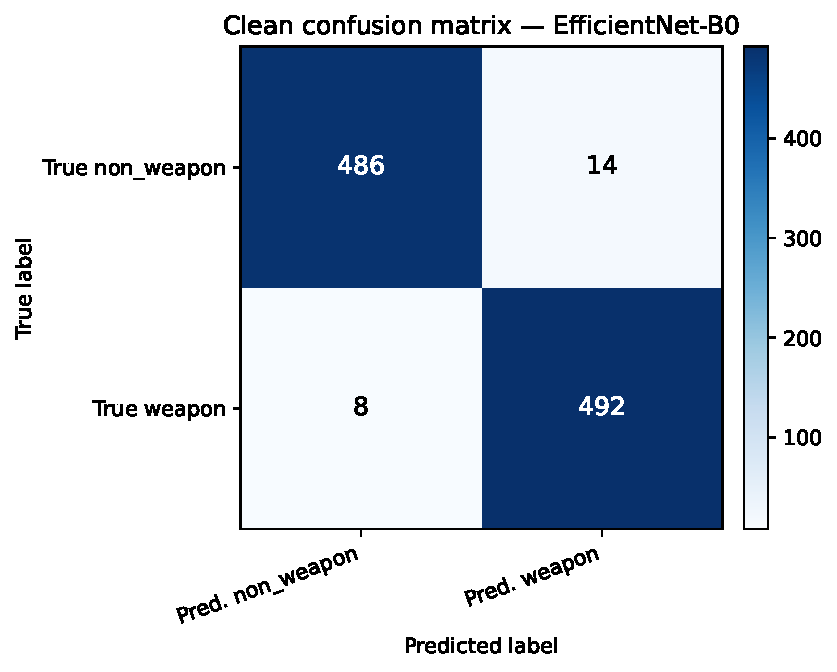
\includegraphics[width=\linewidth]{images/fig_clean_confusion_matrix_efficientnet_b0.pdf}
\end{minipage}
\hfill
\begin{minipage}{0.48\textwidth}
\centering
\small ResNet18

\vspace{0.2em}
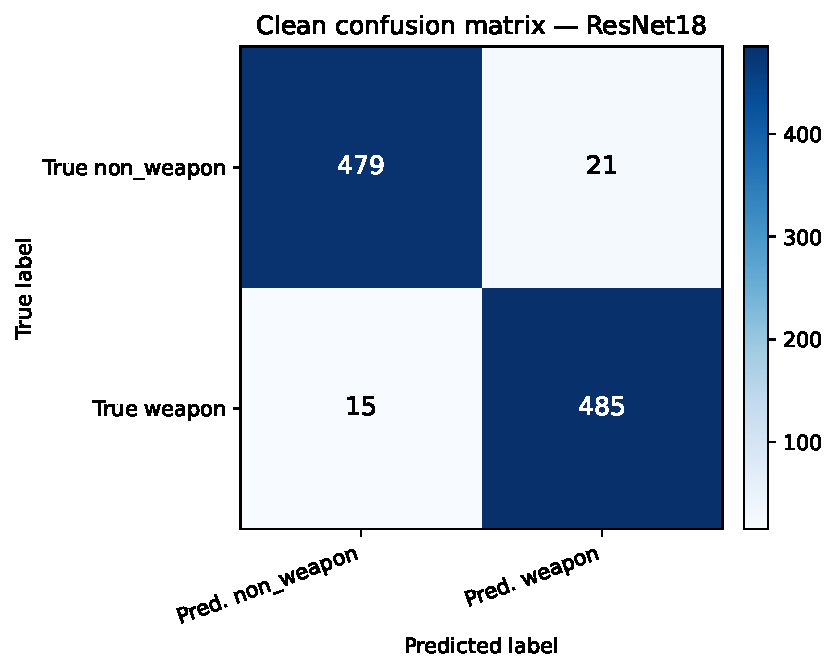
\includegraphics[width=\linewidth]{images/fig_clean_confusion_matrix_resnet18.pdf}
\end{minipage}

\vspace{0.8em}

\begin{minipage}{0.48\textwidth}
\centering
\small \acrshort{clip}

\vspace{0.2em}
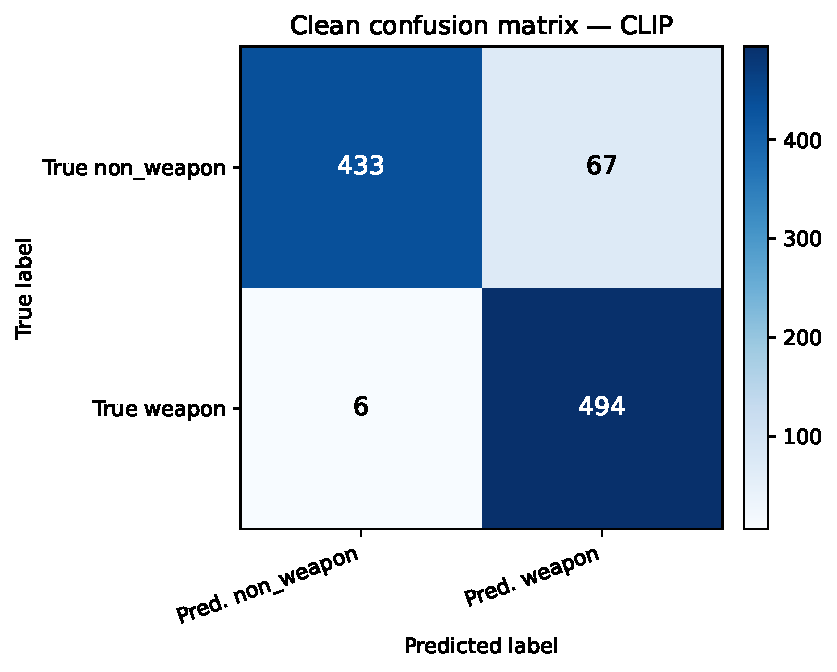
\includegraphics[width=\linewidth]{images/fig_clean_confusion_matrix_clip.pdf}
\end{minipage}

\caption{Confusion matrix clean dei tre modelli proxy sul subset binario. Le righe rappresentano la label reale, mentre le colonne rappresentano la label predetta.}
\label{fig:results-clean-confusion-matrices}
\end{figure}

Dal punto di vista forense, il dato più critico è rappresentato dai falsi
negativi sulla classe \texttt{weapon}. EfficientNet-B0 produce 8 falsi negativi,
ResNet18 ne produce 15, mentre \gls{clip} ne produce 6. Tuttavia, \gls{clip}
produce anche 67 falsi positivi, valore sensibilmente più alto rispetto ai 14 di
EfficientNet-B0 e ai 21 di ResNet18. Ne deriva che il confronto clean non può
essere letto soltanto in termini di accuracy complessiva, ma deve considerare il
diverso bilanciamento tra sensibilità verso la classe investigativamente
rilevante, rischio di segnalazioni improprie e livello di confidenza associato
alle predizioni.

Nel complesso, la baseline clean mostra che i modelli proxy raggiungono
prestazioni elevate in condizioni nominali. Tuttavia, la differenza tra accuracy,
\gls{fpr}, \gls{fnr} e confidenza media evidenzia già in assenza di perturbazioni
un aspetto rilevante per il triage forense: modelli con accuracy simile possono
produrre profili di rischio operativo diversi, soprattutto quando l'errore
riguarda la mancata segnalazione di contenuti \texttt{weapon}, la classificazione
impropria di contenuti \texttt{non\_weapon} come potenzialmente rilevanti oppure
la produzione di predizioni altamente confidenti su casi che richiedono comunque
verifica umana.



% ─────────────────────────────────────────────────────────────────────────────
\section{Out-of-Distribution Behavior and False Positive Risk}
\label{sec:results-ood}
% ─────────────────────────────────────────────────────────────────────────────

La valutazione \gls{ood} analizza il comportamento dei modelli proxy su immagini
che non appartengono al task binario nominale
\texttt{weapon}/\texttt{non\_weapon}. Questi campioni includono contenuti
borderline o fuori distribuzione, quali coltelli, spade, repliche, airsoft,
render sintetici, immagini videoludiche, scene di guerra, mezzi militari,
esplosioni e immagini degradate o anomale. A differenza delle perturbazioni
adversariali e delle trasformazioni anti-forensi, la condizione \gls{ood} non
rappresenta un attacco, ma un rischio operativo realistico: in un workflow
investigativo, immagini ambigue o non pienamente aderenti alle classi operative
del modello possono essere comunque sottoposte ad analisi automatica
\cite{hendrycks2017baseline,liang2018odin,fort2021exploring}.

Le metriche sono aggregate su 2,500 predizioni, ottenute valutando le 500
immagini \gls{ood} attraverso i cinque checkpoint fold-aware di ciascun modello.
Questa scelta mantiene la coerenza con la strategia di valutazione adottata per
il subset binario, pur preservando la separazione concettuale tra campioni
\gls{ood} e task \texttt{weapon}/\texttt{non\_weapon}. Il valore
\emph{weapon rate} indica la quota di campioni \gls{ood} classificati come
\texttt{weapon}; il valore \emph{high-confidence rate} indica invece la quota di
predizioni con confidenza almeno pari a 0.9. In questa sezione, tali valori non
devono essere interpretati come accuracy o errore supervisionato su una terza
classe, ma come indicatori del rischio di assorbimento operativo dei campioni
fuori distribuzione entro una delle due classi del task binario.

\begin{table}[H]
\centering
\scriptsize
\setlength{\tabcolsep}{3.5pt}
\renewcommand{\arraystretch}{1.15}
\caption{Comportamento dei modelli proxy sui campioni \gls{ood}.}
\label{tab:results-ood-behavior}
\begin{tabular}{@{}l r r r r r r r@{}}
\toprule
\textbf{Modello} &
\textbf{Tot.} &
\textbf{Pred. w} &
\textbf{Pred. nw} &
\textbf{W-rate} &
\textbf{Conf.} &
\textbf{HC-count} &
\textbf{HC-rate} \\
\midrule
EfficientNet-B0 & 2,500 & 924 & 1,576 & 0.3696 & 0.8505 & 1,252 & 0.5008 \\
ResNet18 & 2,500 & 1,094 & 1,406 & 0.4376 & 0.8896 & 1,617 & 0.6468 \\
\acrshort{clip} & 2,500 & 2,089 & 411 & 0.8356 & 0.5358 & 0 & 0.0000 \\
\bottomrule
\end{tabular}

\vspace{0.4em}
\footnotesize
\textit{Nota.} \textit{Pred. w} indica le predizioni \texttt{weapon};
\textit{Pred. nw} indica le predizioni \texttt{non\_weapon};
\textit{W-rate} indica la quota di campioni \gls{ood} classificati come
\texttt{weapon}; \textit{Conf.} indica la confidenza media; \textit{HC-count}
indica il numero di predizioni con confidenza almeno pari a 0.9; \textit{HC-rate}
indica la corrispondente quota sul totale delle predizioni \gls{ood}. Il totale
di 2,500 predizioni per modello è ottenuto valutando le 500 immagini \gls{ood}
attraverso ciascuno dei cinque checkpoint fold-aware.
\end{table}


Il valore nullo di \textit{HC-rate} per \gls{clip} non indica assenza di
classificazioni \texttt{weapon} sui campioni \gls{ood}, ma assenza di predizioni
con confidenza pari o superiore alla soglia di alta confidenza fissata a 0.9.
Infatti, \gls{clip} ricondduce alla classe \texttt{weapon} l'83.56\% delle
predizioni \gls{ood}, ma con una confidenza media pari a 0.5358. Questo
comportamento evidenzia una tendenza semantica verso la classe
\texttt{weapon}, non accompagnata però da predizioni ad alta confidenza.


La Figura~\ref{fig:results-ood-weapon-rate-confidence} visualizza il confronto
tra weapon rate, confidenza media e high-confidence rate, mentre la
Figura~\ref{fig:results-ood-confidence-distribution} mostra la distribuzione
delle confidenze predittive sui campioni \gls{ood}.

\begin{figure}[H]
\centering

\includegraphics[width=0.88\textwidth]{images/fig_ood_weapon_rate_and_confidence.pdf}
\caption{Comportamento dei modelli proxy sui campioni \gls{ood}: quota di predizioni \texttt{weapon}, confidenza media e quota di predizioni ad alta confidenza.}
\label{fig:results-ood-weapon-rate-confidence}
\end{figure}

I risultati mostrano tre profili distinti. \gls{clip} classifica come
\texttt{weapon} una quota molto elevata di campioni \gls{ood}, pari a 0.8356,
ma lo fa con una confidenza media contenuta, pari a 0.5358, e senza predizioni
sopra la soglia di alta confidenza. Il valore nullo di high-confidence rate per
\gls{clip} indica infatti che nessuna predizione \gls{ood} supera la soglia di
confidenza 0.9. EfficientNet-B0 e ResNet18, al contrario, classificano come
\texttt{weapon} una quota inferiore di campioni \gls{ood}, rispettivamente pari
a 0.3696 e 0.4376, ma con confidenze medie molto più alte. In particolare,
ResNet18 presenta un high-confidence rate pari a 0.6468, mentre EfficientNet-B0
raggiunge 0.5008.

\begin{figure}[H]
\centering
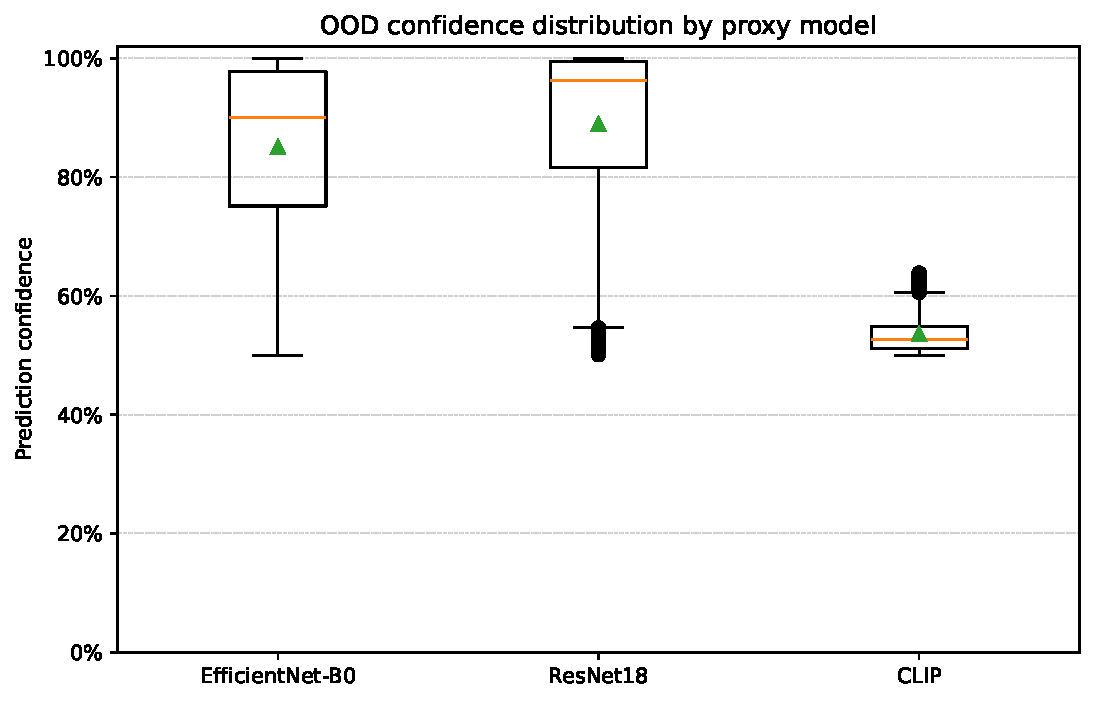
\includegraphics[width=0.82\textwidth]{images/fig_ood_confidence_distribution.pdf}
\caption{Distribuzione della confidenza predittiva sui campioni \gls{ood} per ciascun modello proxy. Il grafico evidenzia una distribuzione più concentrata su valori intermedi per \gls{clip}, rispetto ai due modelli supervisionati.}
\label{fig:results-ood-confidence-distribution}
\end{figure}

La Figura~\ref{fig:results-ood-confidence-distribution} mostra che la
distribuzione delle confidenze di \gls{clip} è più concentrata verso valori
intermedi, mentre EfficientNet-B0 e ResNet18 presentano distribuzioni più
polarizzate verso confidenze alte. Questo dato evidenzia un profilo di rischio
operativo differente: non conta soltanto la frequenza con cui un campione
\gls{ood} viene ricondotto alla classe \texttt{weapon}, ma anche il livello di
confidenza con cui tale assegnazione viene prodotta.

Dal punto di vista forense, questo risultato è rilevante perché evidenzia un
rischio diverso rispetto alla normale misclassificazione binaria. Una predizione
impropria su un campione fuori distribuzione può infatti generare una
segnalazione investigativa non pienamente fondata oppure, al contrario,
rafforzare indebitamente la percezione di rilevanza di un contenuto ambiguo. Il
caso di ResNet18 ed EfficientNet-B0 mostra che un modello può produrre meno
classificazioni \texttt{weapon} su campioni \gls{ood}, ma attribuire a tali
predizioni una confidenza elevata. Il caso di \gls{clip}, invece, mostra un
comportamento opposto: maggiore propensione a classificare come \texttt{weapon},
ma con confidenza più bassa. Questa distinzione è essenziale in un contesto
forense, nel quale la confidenza del sistema non deve essere interpretata come
prova autonoma, ma come informazione ausiliaria soggetta a verifica umana
\cite{guo2017calibration,nist2023airmf}.



% ─────────────────────────────────────────────────────────────────────────────
\section{Anti-Forensic Robustness}
\label{sec:results-antiforensic}
% ─────────────────────────────────────────────────────────────────────────────

La valutazione anti-forense misura la stabilità dei modelli proxy rispetto a
trasformazioni model-agnostic che possono emergere in scenari operativi
realistici. A differenza degli attacchi adversariali, tali trasformazioni non
richiedono accesso al modello target e non sono necessariamente progettate per
massimizzare l'errore di classificazione. Esse simulano invece alterazioni comuni
del contenuto visuale o del file immagine, quali ricompressione,
ridimensionamento, sfocatura, modifica della distribuzione tonale e
normalizzazione del contrasto
\cite{stamm2010anti,yaacoub2021digital,hendrycks2019benchmarking}.

In coerenza con la convenzione definita nella
Sezione~\ref{sec:results-scope}, il drop prestazionale è calcolato come
[
\text{accuracy drop} =
\text{accuracy}\textit{{clean} - \text{accuracy}}{perturbed}.
]
Valori positivi indicano quindi una riduzione della prestazione rispetto alla
baseline clean; valori pari a zero indicano stabilità; valori negativi indicano
un lieve incremento dell'accuracy nella condizione trasformata. Tali incrementi
non devono essere interpretati come prova di robustezza generale, ma come
oscillazioni compatibili con la specifica distribuzione dei campioni trasformati
e con la sensibilità del modello alla trasformazione applicata.

La Tabella~\ref{tab:results-antiforensic-robustness} riporta, per ciascuna
trasformazione, l'accuracy perturbata e l'accuracy drop rispetto alla baseline
clean.

\begin{table}[H]
\centering
\scriptsize
\setlength{\tabcolsep}{3.3pt}
\renewcommand{\arraystretch}{1.15}
\caption{Accuracy perturbata e accuracy drop sotto trasformazioni anti-forensi.}
\label{tab:results-antiforensic-robustness}
\begin{tabular}{@{}l r r r r r r@{}}
\toprule
\textbf{Trasformazione} &
\textbf{\gls{clip} acc.} & \textbf{Drop} &
\textbf{EffNet acc.} & \textbf{Drop} &
\textbf{ResNet acc.} & \textbf{Drop} \\
\midrule
\gls{jpegrecompression} & 0.925 & 0.002 & 0.976 & 0.002 & 0.964 & 0.000 \\
\gls{resampleresize} & 0.929 & -0.002 & 0.976 & 0.002 & 0.963 & 0.001 \\
\gls{gaussianblur} & 0.934 & -0.007 & 0.965 & 0.013 & 0.959 & 0.005 \\
\gls{histogrammodification} & 0.925 & 0.002 & 0.973 & 0.005 & 0.934 & 0.030 \\
\gls{contraststretching} & 0.927 & 0.000 & 0.974 & 0.004 & 0.963 & 0.001 \\
\bottomrule
\end{tabular}

\vspace{0.4em}
\footnotesize
\textit{Nota.} Il drop è definito come
\(\text{accuracy}_{clean}-\text{accuracy}_{perturbed}\). Valori positivi indicano
una degradazione della prestazione; valori negativi indicano un lieve incremento
rispetto alla baseline clean.
\end{table}

La Figura~\ref{fig:results-antiforensic-accuracy-drop-heatmap} visualizza la
stessa valutazione in forma di heatmap, evidenziando la distribuzione del drop
tra modelli e trasformazioni.

\begin{figure}[H]
\centering
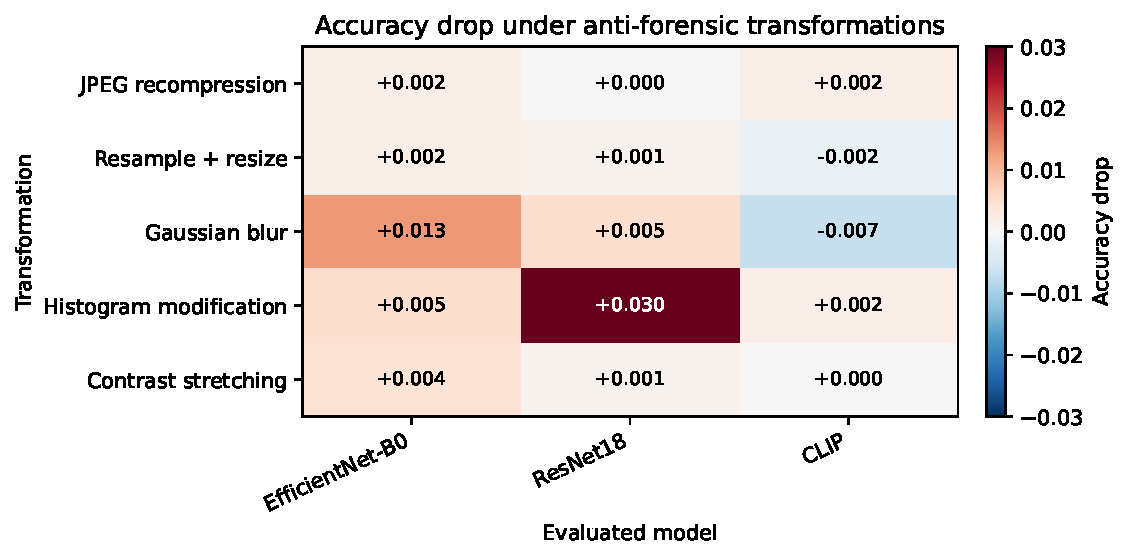
\includegraphics[width=0.88\textwidth]{images/fig_anti_forensic_accuracy_drop_heatmap.pdf}
\caption{Accuracy drop sotto trasformazioni anti-forensi. Il drop è definito come (\text{accuracy}\textit{{clean}-\text{accuracy}}{perturbed}): valori positivi indicano una degradazione della prestazione, mentre valori negativi indicano un lieve incremento rispetto alla baseline clean.}
\label{fig:results-antiforensic-accuracy-drop-heatmap}
\end{figure}

I risultati mostrano che le trasformazioni anti-forensi producono effetti
complessivamente contenuti sui modelli proxy, soprattutto se confrontati con le
perturbazioni adversariali discusse nella Sezione~\ref{sec:results-adversarial}.
EfficientNet-B0 mantiene prestazioni elevate in tutte le condizioni, ma risulta
maggiormente sensibile a \gls{gaussianblur}, con accuracy pari a 0.965 e drop
pari a 0.013. ResNet18 mostra invece la maggiore degradazione in corrispondenza
di \gls{histogrammodification}, con accuracy pari a 0.934 e drop pari a 0.030.
\gls{clip} rimane sostanzialmente stabile, con drop molto contenuti e, in alcuni
casi, lievi incrementi dell'accuracy rispetto alla baseline clean.

La Tabella~\ref{tab:results-antiforensic-operational-errors} riporta alcuni
indicatori operativi aggiuntivi per le condizioni anti-forensi più rilevanti.
Tali valori consentono di distinguere il semplice drop di accuracy dalla natura
degli errori indotti, con particolare attenzione alle transizioni
\texttt{weapon}\(\rightarrow\)\texttt{non\_weapon}, che rappresentano il caso più
critico in un workflow di triage forense.

\begin{table}[H]
\centering
\scriptsize
\setlength{\tabcolsep}{4pt}
\renewcommand{\arraystretch}{1.15}
\caption{Indicatori operativi per le trasformazioni anti-forensi più rilevanti.}
\label{tab:results-antiforensic-operational-errors}
\begin{tabular}{@{}l l r r r r@{}}
\toprule
\textbf{Modello} &
\textbf{Trasformazione} &
\textbf{Induced errors} &
\textbf{Confidence shift} &
\textbf{W\(\rightarrow\)NW} &
\textbf{NW\(\rightarrow\)W} \\
\midrule
EfficientNet-B0 & \gls{gaussianblur} & 17 & -0.0099 & 17 & 0 \\
ResNet18 & \gls{histogrammodification} & 39 & -0.0157 & 23 & 16 \\
\acrshort{clip} & \gls{histogrammodification} & 13 & -0.0037 & 6 & 7 \\
\bottomrule
\end{tabular}

\vspace{0.4em}
\footnotesize
\textit{Nota.} \textit{Induced errors} indica il numero di errori introdotti
rispetto alle predizioni clean corrette; \textit{Confidence shift} indica la
variazione media della confidenza rispetto alla condizione clean;
W\(\rightarrow\)NW indica transizioni da \texttt{weapon} a
\texttt{non\_weapon}; NW\(\rightarrow\)W indica transizioni da
\texttt{non\_weapon} a \texttt{weapon}.
\end{table}

La trasformazione più critica per EfficientNet-B0 è \gls{gaussianblur}, che
introduce 17 errori rispetto alle predizioni clean corrette, tutti nella direzione
\texttt{weapon}\(\rightarrow\)\texttt{non\_weapon}. Per ResNet18, la condizione
più rilevante è \gls{histogrammodification}, che introduce 39 errori, di cui 23
nella direzione \texttt{weapon}\(\rightarrow\)\texttt{non\_weapon} e 16 nella
direzione opposta. Per \gls{clip}, gli effetti restano più contenuti, ma
\gls{histogrammodification} introduce comunque 13 errori rispetto alla baseline
clean, distribuiti tra entrambe le direzioni di errore.

Dal punto di vista operativo, questi risultati non devono essere considerati
trascurabili soltanto perché i drop sono inferiori a quelli osservati nelle
condizioni adversariali. Le trasformazioni anti-forensi sono infatti più
facilmente riconducibili a condizioni realistiche di circolazione, compressione,
modifica e ricondivisione delle immagini. In un workflow di \gls{df}, anche una
riduzione limitata della prestazione può diventare rilevante quando riguarda
contenuti investigativamente sensibili o quando si combina con altri fattori di
incertezza, quali bassa qualità dell'immagine, contesto ambiguo o assenza di
verifica manuale sistematica.



% ─────────────────────────────────────────────────────────────────────────────
\section{Adversarial Robustness}
\label{sec:results-adversarial}
% ─────────────────────────────────────────────────────────────────────────────

La valutazione adversarial misura la risposta dei modelli proxy a perturbazioni
progettate per alterare il comportamento del classificatore
\cite{szegedy2014intriguing,goodfellow2015explaining,biggio2018wild}. Nel
contesto della presente tesi, tali perturbazioni non sono analizzate come fine
autonomo di \gls{advml}, ma come stressor sperimentali utili a valutare
l'affidabilità operativa di sistemi \gls{ai}-based in scenari forensi.
L'interesse principale non riguarda quindi soltanto la capacità dell'attacco di
ridurre l'accuracy, ma il rischio che immagini della classe \texttt{weapon}
vengano riclassificate come \texttt{non\_weapon}, generando falsi negativi
potenzialmente critici in un processo di triage investigativo.

Gli attacchi model-dependent sono generati contro EfficientNet-B0. Questa scelta
riflette uno scenario white-box nel quale l'avversario dispone di accesso pieno a
un singolo modello target; la trasferibilità verso architetture differenti viene
quindi valutata empiricamente, anziché assunta a priori
\cite{biggio2018wild,nowroozi2021survey,barni2018cf}. \gls{colorshift} è invece
trattato come perturbazione model-agnostic di stile adversarial.

In coerenza con la convenzione definita nella
Sezione~\ref{sec:results-scope}, il drop prestazionale è calcolato come
[
\text{accuracy drop} =
\text{accuracy}\textit{{clean} - \text{accuracy}}{perturbed}.
]
Valori positivi indicano quindi una degradazione della prestazione rispetto alla
baseline clean; valori pari a zero indicano stabilità; valori negativi indicano
un lieve incremento dell'accuracy nella condizione perturbata. Tali incrementi
non vengono interpretati come prova di robustezza generale, ma come oscillazioni
dipendenti dalla distribuzione dei campioni e dalla specifica trasferibilità
delle perturbazioni generate contro il modello target.

La Tabella~\ref{tab:results-adversarial-robustness} riporta, per ciascuna
famiglia di perturbazioni, l'accuracy perturbata e l'accuracy drop rispetto alla
baseline clean.

\begin{table}[H]
\centering
\scriptsize
\setlength{\tabcolsep}{3.3pt}
\renewcommand{\arraystretch}{1.15}
\caption{Accuracy perturbata e accuracy drop sotto perturbazioni adversariali.}
\label{tab:results-adversarial-robustness}
\begin{tabular}{@{}l r r r r r r@{}}
\toprule
\textbf{Perturbazione} &
\textbf{\gls{clip} acc.} & \textbf{Drop} &
\textbf{EffNet acc.} & \textbf{Drop} &
\textbf{ResNet acc.} & \textbf{Drop} \\
\midrule
\gls{fgsm} & 0.914 & 0.013 & 0.575 & 0.403 & 0.918 & 0.046 \\
\gls{superdeepfool} & 0.926 & 0.001 & 0.931 & 0.047 & 0.964 & 0.000 \\
\gls{sigmazero} & 0.944 & -0.017 & 0.015 & 0.963 & 0.968 & -0.004 \\
\gls{onepixel} & 0.928 & -0.001 & 0.976 & 0.002 & 0.963 & 0.001 \\
\gls{colorshift} & 0.925 & 0.002 & 0.977 & 0.001 & 0.963 & 0.001 \\
\bottomrule
\end{tabular}

\vspace{0.4em}
\footnotesize
\textit{Nota.} Il drop è definito come
(\text{accuracy}\textit{{clean}-\text{accuracy}}{perturbed}). Valori positivi indicano
una degradazione della prestazione; valori negativi indicano un lieve incremento
rispetto alla baseline clean.
\end{table}

La Figura~\ref{fig:results-adversarial-accuracy-drop-heatmap} visualizza la
stessa valutazione in forma di heatmap. La concentrazione dei valori più elevati
nella colonna EfficientNet-B0 riflette il fatto che gli attacchi model-dependent
sono stati generati contro tale modello.

\begin{figure}[H]
\centering
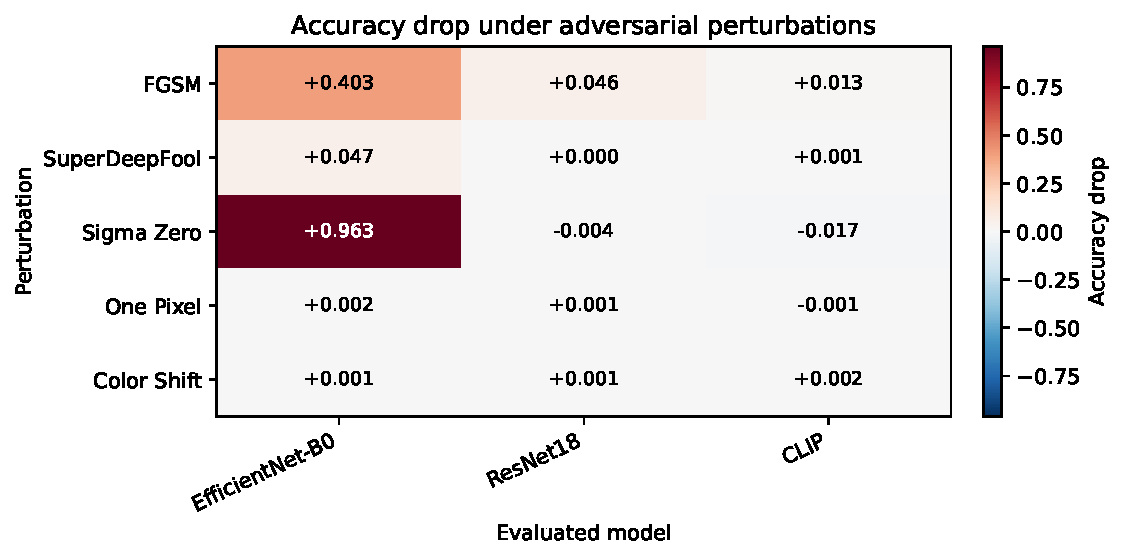
\includegraphics[width=0.88\textwidth]{images/fig_adversarial_accuracy_drop_heatmap.pdf}
\caption{Accuracy drop sotto perturbazioni adversariali. Il drop è definito come (\text{accuracy}\textit{{clean}-\text{accuracy}}{perturbed}). La degradazione più marcata riguarda EfficientNet-B0 sotto \gls{sigmazero}, evidenziando la vulnerabilità del modello nello scenario white-box considerato.}
\label{fig:results-adversarial-accuracy-drop-heatmap}
\end{figure}

Il risultato più critico riguarda EfficientNet-B0 sotto \gls{sigmazero}, dove
l'accuracy passa da 0.978 a 0.015, con un accuracy drop pari a 0.963. Tale valore
indica una degradazione quasi completa della capacità classificativa del modello,
limitata tuttavia alla configurazione white-box in cui l'attacco è ottimizzato
direttamente contro EfficientNet-B0 con accesso pieno ai suoi parametri. In
termini operativi, questo risultato corrisponde a un comportamento incompatibile
con un uso non verificato del modello per il triage automatico di immagini
contenenti armi: la baseline clean più elevata tra i proxy non impedisce infatti
una forte degradazione quando il modello è esposto a perturbazioni ottimizzate
contro di esso.

Anche \gls{fgsm}, generato contro EfficientNet-B0, produce un degrado rilevante,
riducendo l'accuracy a 0.575 e determinando un accuracy drop pari a 0.403.
\gls{superdeepfool} produce invece un effetto più contenuto sullo stesso modello,
con accuracy pari a 0.931 e drop pari a 0.047. \gls{onepixel} e \gls{colorshift}
producono variazioni marginali su EfficientNet-B0, rispettivamente pari a 0.002 e
0.001.

Il confronto con ResNet18 e \gls{clip} mostra che il trasferimento degli attacchi
generati contro EfficientNet-B0 non produce una degradazione equivalente sugli
altri modelli. ResNet18 subisce il drop maggiore sotto \gls{fgsm}, pari a 0.046,
mentre rimane sostanzialmente stabile rispetto a \gls{superdeepfool},
\gls{onepixel}, \gls{sigmazero} e \gls{colorshift}. \gls{clip} mostra variazioni
ancora più contenute, con il peggioramento massimo pari a 0.013 sotto
\gls{fgsm}. In alcuni casi, come \gls{sigmazero}, l'accuracy perturbata di
\gls{clip} e ResNet18 risulta lievemente superiore alla rispettiva baseline
clean; tale effetto viene interpretato come oscillazione specifica della
distribuzione valutata e non come evidenza di robustezza generale.

La Tabella~\ref{tab:results-adversarial-operational-errors} riporta indicatori
operativi aggiuntivi per le condizioni adversariali più rilevanti. Tali valori
permettono di distinguere il drop di accuracy dalla direzione degli errori
indotti, con particolare attenzione alle transizioni
\texttt{weapon}\(\rightarrow\)\texttt{non\_weapon}.

\begin{table}[H]
\centering
\scriptsize
\setlength{\tabcolsep}{3.5pt}
\renewcommand{\arraystretch}{1.15}
\caption{Indicatori operativi per le perturbazioni adversariali più rilevanti.}
\label{tab:results-adversarial-operational-errors}
\begin{tabular}{@{}l l r r r r r@{}}
\toprule
\textbf{Modello} &
\textbf{Perturbazione} &
\textbf{Induced errors} &
\textbf{ASR} &
\textbf{Confidence shift} &
\textbf{W\(\rightarrow\)NW} &
\textbf{NW\(\rightarrow\)W} \\
\midrule
EfficientNet-B0 & \gls{sigmazero} & 963 & 0.9847 & -0.2578 & 489 & 474 \\
EfficientNet-B0 & \gls{fgsm} & 406 & 0.4151 & -0.1246 & 321 & 85 \\
EfficientNet-B0 & \gls{superdeepfool} & 47 & 0.0481 & -0.3063 & 0 & 47 \\
ResNet18 & \gls{fgsm} & 47 & 0.0488 & -0.0230 & 27 & 20 \\
\acrshort{clip} & \gls{fgsm} & 23 & 0.0248 & -0.0043 & 8 & 15 \\
\bottomrule
\end{tabular}

\vspace{0.4em}
\footnotesize
\textit{Nota.} \textit{Induced errors} indica il numero di errori introdotti
rispetto alle predizioni clean corrette; \textit{ASR} indica l'attack success
rate calcolato rispetto ai campioni correttamente classificati in condizioni
clean; \textit{Confidence shift} indica la variazione media della confidenza
rispetto alla condizione clean; W\(\rightarrow\)NW indica transizioni da
\texttt{weapon} a \texttt{non\_weapon}; NW\(\rightarrow\)W indica transizioni da
\texttt{non\_weapon} a \texttt{weapon}.
\end{table}

La lettura degli errori indotti conferma la criticità operativa dello scenario
EfficientNet-B0 sotto \gls{sigmazero}: 963 errori vengono introdotti rispetto
alle predizioni clean corrette, con 489 transizioni
\texttt{weapon}\(\rightarrow\)\texttt{non\_weapon}. Questo aspetto è più
rilevante della sola accuracy, poiché descrive direttamente il rischio di
mancata segnalazione di contenuti appartenenti alla classe investigativamente
rilevante. Anche \gls{fgsm} produce un effetto significativo su EfficientNet-B0,
con 406 errori indotti e 321 transizioni
\texttt{weapon}\(\rightarrow\)\texttt{non\_weapon}. Per ResNet18 e \gls{clip},
gli effetti trasferiti risultano più contenuti, ma non nulli.

Dal punto di vista forense, la vulnerabilità di EfficientNet-B0 a perturbazioni
come \gls{sigmazero} e \gls{fgsm} evidenzia un rischio operativo significativo:
un sistema apparentemente molto accurato in condizioni clean può degradare in
modo drastico quando esposto a input manipolati in modo deliberato. Questo
rafforza la necessità di non interpretare l'output di un classificatore
\gls{ai}-based come evidenza autonoma, ma come supporto al triage da sottoporre
a verifica, tracciamento e valutazione nel contesto complessivo dell'indagine.



% ─────────────────────────────────────────────────────────────────────────────
\section{Forensic Evaluation Bundle Composition and Black-Box Readiness}
\label{sec:results-bundle}
% ─────────────────────────────────────────────────────────────────────────────

Il forensic evaluation bundle costituisce il livello di collegamento tra la
valutazione sperimentale controllata dei modelli proxy e la successiva
valutazione black-box degli strumenti commerciali e dei software selezionati. Il
bundle è progettato per fornire ai tool un input cieco e semanticamente neutro,
preservando separatamente le informazioni necessarie per il matching, la
normalizzazione degli export e l'audit dei risultati
\cite{casey2011digital,nist2006guide,iso27041,iso27042,swgde2014validation}.

A differenza della composizione generale del corpus sperimentale riportata nella
Sezione~\ref{sec:results-scope}, la
Tabella~\ref{tab:results-bundle-operational-layout} descrive il bundle dal punto
di vista operativo, distinguendo tra contenuto sottoposto ai tool, naming cieco e
ruolo dei metadati nella fase di audit. Il totale è pari a 11,500 file,
comprendenti 1000 campioni clean, 500 campioni \gls{ood}, 5000 campioni
adversariali e 5000 campioni anti-forensi.

\begin{table}[H]
\centering
\scriptsize
\renewcommand{\arraystretch}{1.15}
\setlength{\tabcolsep}{4pt}
\caption{Vista operativa del forensic evaluation bundle per la valutazione black-box.}
\label{tab:results-bundle-operational-layout}
\begin{tabularx}{\textwidth}{@{}l r l X@{}}
\toprule
\textbf{Componente} &
\textbf{File} &
\textbf{Input cieco} &
\textbf{Ruolo dei metadati} \\
\midrule

Clean &
1000 &
\texttt{bundle\_*.jpg} &
Conserva la corrispondenza con il subset binario originale e con la label
\texttt{weapon}/\texttt{non\_weapon}. \\

\gls{ood} &
500 &
\texttt{bundle\_*.jpg} &
Preserva la distinzione tra campioni fuori distribuzione e task binario
nominale. \\

Adversarial &
5000 &
\texttt{bundle\_*.jpg} &
Registra famiglia di attacco, nome della perturbazione, modello target e
immagine sorgente. \\

Anti-forensic &
5000 &
\texttt{bundle\_*.jpg} &
Registra trasformazione applicata, immagine sorgente e mapping verso il
campione clean corrispondente. \\

\midrule
\textbf{Totale} &
\textbf{11,500} &
\texttt{bundle\_*.jpg} &
Abilita matching, normalizzazione post-export e audit hash-based. \\
\bottomrule
\end{tabularx}
\end{table}

La costruzione del bundle segue due viste complementari. La prima è una
directory cieca destinata agli strumenti valutati, nella quale i file sono
rinominati con identificativi neutri del tipo \texttt{bundle\_000001.jpg}. La
seconda è una vista strutturata di audit, riservata al ricercatore, nella quale
sono preservate le informazioni semantiche e sperimentali necessarie alla
verifica. Per la valutazione black-box, gli strumenti devono importare
esclusivamente la directory:

\begin{center}
\codepath{datasets/forensic_evaluation_bundle/blind_tool_input/files}
\end{center}

e non devono importare né la directory \codepath{metadata/} né la directory
\codepath{structured_audit_view/}. Questa separazione riduce il rischio di bias
indotto dai nomi dei file, dai path, dalle classi, dai nomi degli attacchi o
dalla struttura degli split.

Il bundle preserva la tracciabilità attraverso manifest separati contenenti, per
ciascun file, identificativo del bundle, nome cieco, tipo di campione, famiglia e
nome della perturbazione, fold, label finale, dataset sorgente, identificativo
dell'immagine originale, path sorgente, path cieco, path strutturato, hash
\gls{sha256}, hash \gls{md5}, dimensione del file ed estensione. Tale struttura
consente di collegare ogni output esportato da un tool al corrispondente
artefatto sperimentale senza esporre al tool la ground truth durante la fase di
importazione.

I controlli di consistenza hanno verificato che gli identificativi del bundle
siano univoci, che gli hash \gls{sha256} effettivi siano univoci, che gli hash
calcolati corrispondano a quelli riportati nel manifest quando disponibili, che i
path ciechi siano semanticamente neutri e che i metadati sperimentali siano
separati dall'input operativo dei tool. Questi controlli sono essenziali per
rendere il bundle idoneo alla valutazione black-box, poiché permettono di
distinguere tra errori di classificazione, file non processati, output non
categorizzati, limiti del formato di export e problemi di matching
\cite{iso27041,iso27042,iso27043,swgde2014validation}.

In sintesi, il forensic evaluation bundle consente di passare da una valutazione
proxy completamente controllata a una valutazione più vicina al contesto
operativo degli strumenti black-box. La sua funzione non è soltanto organizzativa,
ma metodologica: preserva la riproducibilità dell'esperimento e riduce
l'esposizione dei tool a informazioni semantiche non necessarie. Al tempo stesso,
abilita una normalizzazione post-export basata su identificativi e hash
verificabili, condizione necessaria per distinguere errori di classificazione
genuini da artefatti del processo di export o da limiti del mapping operativo.



% ─────────────────────────────────────────────────────────────────────────────
\section{Commercial Forensic Tools Evaluation}
\label{sec:results-commercial}
% ─────────────────────────────────────────────────────────────────────────────

La valutazione degli strumenti commerciali rappresenta il livello black-box della
pipeline sperimentale. A differenza dei modelli proxy analizzati nelle sezioni
precedenti, per tali strumenti non sono disponibili architettura del modello,
dataset di addestramento, soglie decisionali, preprocessing interno o logica
completa di classificazione. La valutazione si basa quindi esclusivamente sugli
output osservabili prodotti dai tool, sui tag assegnati, sulle categorie esportate
e sul matching tra i file del forensic evaluation bundle e la ground truth
sperimentale.

Il confronto commerciale include tre sistemi finali. \gls{magnetaxiomtool} con
\gls{magnetai} è valutato come piattaforma forense commerciale dotata di
funzionalità \gls{ai}-based di categorizzazione delle immagini.
\gls{excirefoto2025} è valutato come software standalone general-purpose di
semantic retrieval con funzionalità \gls{ai}-based, non come prodotto sviluppato
esclusivamente per finalità forensi. \gls{cellebriteinseyets} è valutato come
tool commerciale black-box di media analysis, mediante output osservabili
esportati e normalizzati dall'ambiente \texttt{Cellebrite Physical Analyzer
10.9.0.3029}. In questo contesto, \gls{ufed} non viene trattato come
classificatore immagini, ma solo come eventuale componente dell'ecosistema
Cellebrite di acquisizione e gestione dei dati.

Per evitare che gli strumenti potessero utilizzare informazioni semantiche
derivate dai nomi dei file, dai path o dalla struttura delle cartelle, la
valutazione è stata condotta utilizzando la vista cieca del forensic evaluation
bundle. I file sono stati importati con nomi neutri del tipo
\texttt{bundle\_*.jpg}, mentre le informazioni relative a classe, sorgente, fold,
attacco, trasformazione, hash e ground truth sono state mantenute separate nei
manifest di audit. Dopo l'elaborazione, gli output esportati sono stati
normalizzati e ricondotti ai campioni originali tramite identificativi del bundle
e hash \gls{sha256}/\gls{md5}. Questa impostazione consente di distinguere tra
immagini correttamente segnalate, immagini non segnalate, falsi negativi sulla
classe \texttt{weapon}, falsi positivi sulla classe \texttt{non\_weapon}, output
non interpretabili e comportamento sui campioni \gls{ood}.

La Tabella~\ref{tab:results-commercial-overview} riporta una sintesi comparativa
delle metriche aggregate dei sistemi commerciali e delle configurazioni
operative considerate. Per \gls{excirefoto2025}, le tre righe corrispondono alle
configurazioni \texttt{D20}, \texttt{D50} e \texttt{D80} del parametro
\texttt{Distance limit}. La configurazione \texttt{D50} viene utilizzata come
riferimento principale nelle discussioni comparative, poiché rappresenta il
compromesso intermedio tra configurazione restrittiva e configurazione
permissiva.

\begin{table}[H]
\centering
\scriptsize
\renewcommand{\arraystretch}{1.15}
\setlength{\tabcolsep}{3.4pt}
\caption{Sintesi aggregata della valutazione black-box dei sistemi commerciali.}
\label{tab:results-commercial-overview}
\begin{tabular}{@{}l r r r r r r r@{}}
\toprule
\textbf{Sistema} &
\textbf{Matched} &
\textbf{Acc.} &
\textbf{Bal.} &
\textbf{R\textsubscript{w}} &
\textbf{\acrshort{fnr}} &
\textbf{\acrshort{fpr}} &
\textbf{OOD W-rate} \\
\midrule
\gls{magnetaxiomtool}/\gls{magnetai}
& 11,500 & 0.933 & 0.933 & 0.901 & 0.099 & 0.035 & 0.360 \\

\gls{excirefoto2025} \texttt{D20}
& 11,500 & 0.911 & 0.911 & 0.857 & 0.143 & 0.036 & 0.238 \\

\gls{excirefoto2025} \texttt{D50}
& 11,500 & 0.925 & 0.925 & 0.949 & 0.051 & 0.099 & 0.340 \\

\gls{excirefoto2025} \texttt{D80}
& 11,500 & 0.887 & 0.887 & 0.981 & 0.019 & 0.207 & 0.522 \\

\gls{cellebriteinseyets}
& 11,500 & 0.958 & 0.958 & 0.958 & 0.042 & 0.042 & 0.292 \\
\bottomrule
\end{tabular}

\vspace{0.4em}
\footnotesize
\textit{Nota.} \textit{Matched} indica il numero di file del forensic evaluation
bundle ricondotti a un output normalizzato. \textit{Acc.} indica l'accuracy sul
task binario interpretabile; \textit{Bal.} indica la balanced accuracy;
(R\_w) indica il recall per la classe \texttt{weapon}; \gls{fnr} e \gls{fpr}
indicano rispettivamente false negative rate e false positive rate; \textit{OOD
W-rate} indica la quota di campioni \gls{ood} ricondotti operativamente alla
classe \texttt{weapon}. Le metriche binarie sono calcolate sui campioni
\texttt{weapon}/\texttt{non\_weapon}; i campioni \gls{ood} sono analizzati
separatamente.
\end{table}

La lettura della Tabella~\ref{tab:results-commercial-overview} richiede cautela.
Le metriche non descrivono l'accuratezza interna dei sistemi commerciali in senso
assoluto, ma il comportamento osservato dopo la normalizzazione degli output nel
task operativo \texttt{weapon}/\texttt{non\_weapon}. In particolare, il caso di
\gls{excirefoto2025} mostra chiaramente l'effetto della soglia di retrieval:
\texttt{D20} riduce il tasso di falsi positivi e il weapon flag rate sui campioni
\gls{ood}, ma aumenta i falsi negativi; \texttt{D80} massimizza il recall sulla
classe \texttt{weapon}, ma incrementa in modo marcato i falsi positivi e le
segnalazioni \texttt{weapon} sui campioni \gls{ood}. \texttt{D50} rappresenta
pertanto una configurazione intermedia, utile per il confronto operativo con
\gls{magnetai} e \gls{cellebriteinseyets}.

Nel complesso, questa sezione introduce il livello black-box della valutazione.
Le sottosezioni successive analizzano separatamente i risultati di
\gls{magnetaxiomtool}/\gls{magnetai}, \gls{excirefoto2025} e
\gls{cellebriteinseyets}, distinguendo prestazioni clean, comportamento sugli
input perturbati, rischio di falsi negativi sulla classe \texttt{weapon} e weapon
flag rate sui campioni \gls{ood}.


La normalizzazione degli export commerciali è stata condotta separatamente per
ciascuno strumento, preservando la distinzione tra categorie native, tag
proprietari, risultati di semantic retrieval e predizioni operative ricondotte al
task \texttt{weapon}/\texttt{non\_weapon}. Per
\gls{magnetaxiomtool}/\gls{magnetai}, il tag \texttt{Possible weapons} è stato
interpretato come segnale operativo positivo per la classe \texttt{weapon}. Per
\gls{excirefoto2025}, la normalizzazione è stata effettuata su tre configurazioni
distinte del parametro \texttt{Distance limit}, indicate come \texttt{D20},
\texttt{D50} e \texttt{D80}; tali configurazioni non rappresentano ripetizioni
dello stesso esperimento, ma tre diversi profili di retrieval, rispettivamente
restrittivo, intermedio e permissivo. Per \gls{cellebriteinseyets}, le
classificazioni osservabili esportate dall'ambiente \texttt{Cellebrite Physical
Analyzer 10.9.0.3029} sono state ricodificate nel task operativo
\texttt{weapon}/\texttt{non\_weapon}. In questo contesto, \gls{ufed} non viene
trattato come classificatore immagini, ma solo come eventuale componente
dell'ecosistema Cellebrite di acquisizione e gestione dei dati.

Le sottosezioni successive analizzano separatamente i risultati dei tre sistemi
finali inclusi nella valutazione commerciale: \gls{magnetaxiomtool}/\gls{magnetai},
\gls{excirefoto2025} e \gls{cellebriteinseyets}.



% ─────────────────────────────────────────────────────────────────────────────
\subsection{Magnet AXIOM / Magnet.AI Results}
\label{subsec:results-magnet}
% ─────────────────────────────────────────────────────────────────────────────

La valutazione di \gls{magnetaxiomtool}/\gls{magnetai} costituisce il primo
risultato black-box commerciale consolidato della pipeline. Gli output prodotti
dal tool sono stati normalizzati mappando il tag \texttt{Possible weapons} come
predizione operativa positiva per la classe \texttt{weapon}; l'assenza di tale
tag è stata invece ricondotta alla predizione negativa
\texttt{non\_weapon}. Questa ricodifica consente di confrontare l'output
osservabile del tool con la ground truth sperimentale del forensic evaluation
bundle, senza assumere accesso alla logica decisionale interna del modulo
proprietario.

La normalizzazione ha prodotto un matching completo tra export del tool e
forensic evaluation bundle: tutte le 11,500 immagini sono state ricondotte a un
identificativo del bundle e nessuna riga è rimasta non mappata. Le metriche
binarie sono calcolate sulle 11,000 immagini appartenenti alle classi operative
\texttt{weapon} e \texttt{non\_weapon}; le 500 immagini \gls{ood} sono invece
analizzate separatamente mediante il weapon flag rate.

\begin{table}[H]
\centering
\caption{Sintesi della normalizzazione dell'export \gls{magnetaxiomtool}/\gls{magnetai}.}
\label{tab:results-magnet-normalization-summary}
\small
\begin{tabular}{lr}
\toprule
\textbf{Elemento} & \textbf{Valore} \\
\midrule
Immagini nel forensic evaluation bundle & 11,500 \\
Righe matched & 11,500 \\
Righe unmatched & 0 \\
Righe binarie interpretabili & 11,000 \\
Campioni \gls{ood} analizzati separatamente & 500 \\
Output non interpretabili / unknown & 0 \\
Predizioni operative positive sul bundle completo & 5,329 \\
Predizioni operative negative sul bundle completo & 6,171 \\
\bottomrule
\end{tabular}
\end{table}

La Tabella~\ref{tab:results-magnet-global-metrics} riporta le metriche
complessive di \gls{magnetai} sul task binario
\texttt{weapon}/\texttt{non\_weapon}. Il tool raggiunge un'accuracy pari a
0.933 e una precisione sulla classe \texttt{weapon} pari a 0.963. Tuttavia, il
recall sulla classe \texttt{weapon} è pari a 0.901, con un \gls{fnr} pari a
0.099: 542 immagini appartenenti alla classe \texttt{weapon} non sono state
segnalate come \texttt{Possible weapons}.

\begin{table}[H]
\centering
\caption{Prestazioni complessive di \gls{magnetai} sul task binario \texttt{weapon}/\texttt{non\_weapon}.}
\label{tab:results-magnet-global-metrics}
\small
\begin{tabular}{lr}
\toprule
\textbf{Metrica} & \textbf{Valore} \\
\midrule
Accuracy & 0.933 \\
Balanced accuracy & 0.933 \\
Precision \texttt{weapon} & 0.963 \\
Recall \texttt{weapon} & 0.901 \\
F1 \texttt{weapon} & 0.931 \\
False negative rate & 0.099 \\
False positive rate & 0.035 \\
True positives & 4,958 \\
True negatives & 5,309 \\
False positives & 191 \\
False negatives & 542 \\
\bottomrule
\end{tabular}

\vspace{0.4em}
\footnotesize
\textit{Nota.} Le metriche sono calcolate sulle 11,000 immagini appartenenti al
task binario \texttt{weapon}/\texttt{non\_weapon}. Il valore aggregato non
corrisponde alla media aritmetica tra clean e perturbed, poiché il bundle include
1,000 immagini clean e 10,000 immagini perturbate.
\end{table}

La nota riportata nella Tabella~\ref{tab:results-magnet-global-metrics}
evidenzia che il valore aggregato è influenzato dalla composizione del bundle,
nel quale le immagini perturbate sono numericamente prevalenti rispetto ai
campioni clean. Le metriche complessive devono quindi essere lette insieme alla
disaggregazione per condizione sperimentale riportata nella
Tabella~\ref{tab:results-magnet-condition-metrics}.

\begin{table}[H]
\centering
\caption{Comportamento di \gls{magnetai} per condizione sperimentale.}
\label{tab:results-magnet-condition-metrics}
\small
\begin{tabularx}{\textwidth}{@{}l r r r r X@{}}
\toprule
\textbf{Condizione} &
\textbf{Accuracy} &
\textbf{Recall weapon} &
\textbf{\gls{fnr}} &
\textbf{\gls{fpr}} &
\textbf{Nota operativa} \\
\midrule

Clean &
0.950 &
0.930 &
0.070 &
0.030 &
Baseline commerciale su 1,000 immagini non perturbate. \\

Perturbed &
0.932 &
0.899 &
0.101 &
0.035 &
Valori calcolati su 10,000 immagini perturbate: 5,000 adversariali e 5,000
anti-forensi. Il degrado principale riguarda l'aumento dei falsi negativi sulla
classe \texttt{weapon}. \\

Adversarial &
0.923 &
0.884 &
0.116 &
0.038 &
Prestazione aggregata sulle 5 famiglie adversariali considerate. \\

Anti-forensic &
0.940 &
0.913 &
0.087 &
0.032 &
Prestazione aggregata sulle 5 trasformazioni anti-forensi considerate. \\

\gls{ood} &
-- &
-- &
-- &
-- &
Weapon flag rate pari a 0.360: 180 immagini \gls{ood} su 500 sono state
segnalate come \texttt{Possible weapons}. Le metriche binarie standard non sono
applicabili. \\

\bottomrule
\end{tabularx}
\end{table}

La disaggregazione per condizione mostra che gli attacchi adversariali producono
un impatto più marcato rispetto alle trasformazioni anti-forensi. Il \gls{fnr}
aggregato sulle condizioni adversariali è pari a 0.116, contro 0.087 per le
trasformazioni anti-forensi. Questo risultato indica che, nel caso di
\gls{magnetai}, le perturbazioni progettate per interferire con il comportamento
del classificatore producono un aumento più rilevante dei falsi negativi rispetto
alle trasformazioni realistiche di degradazione o manipolazione dell'immagine.

Il comportamento sulle immagini \gls{ood} è rilevante per il workflow di triage.
Le immagini fuori distribuzione non appartengono al task binario
\texttt{weapon}/\texttt{non\_weapon} e non devono quindi essere interpretate come
errori classici di classificazione. Tuttavia, il fatto che 180 immagini
\gls{ood} su 500 siano state segnalate come \texttt{Possible weapons} indica che
il modulo automatico può assegnare rilevanza investigativa a contenuti
semanticamente ambigui o non appartenenti alla distribuzione attesa.

A differenza dei modelli proxy, \gls{magnetai} non esporta valori di confidenza
numerici associati alle singole predizioni. La classificazione osservabile si
basa esclusivamente sulla presenza o assenza del tag \texttt{Possible weapons},
senza indicazione quantitativa del grado di certezza. Questa caratteristica
preclude il confronto diretto con le distribuzioni di confidenza dei modelli
proxy e costituisce un limite operativo alla tracciabilità interpretativa
dell'output.

La Tabella~\ref{tab:results-magnet-attack-metrics} riporta il comportamento di
\gls{magnetai} rispetto a tutte le perturbazioni considerate nel forensic
evaluation bundle. Tra gli attacchi adversariali, \gls{fgsm} costituisce la
condizione più critica per il tool, con accuracy pari a 0.867, recall sulla
classe \texttt{weapon} pari a 0.808 e \gls{fnr} pari a 0.192. Tra le
trasformazioni anti-forensi, \gls{gaussianblur} produce il valore di \gls{fnr}
più elevato, pari a 0.120.

\begin{table}[H]
\centering
\caption{Prestazioni di \gls{magnetai} nelle condizioni adversariali e anti-forensi.}
\label{tab:results-magnet-attack-metrics}
\scriptsize
\renewcommand{\arraystretch}{1.12}
\setlength{\tabcolsep}{4pt}
\begin{tabular}{@{}l l r r r r r r@{}}
\toprule
\textbf{Famiglia} &
\textbf{Condizione} &
\textbf{Accuracy} &
\textbf{Recall} &
\textbf{\gls{fnr}} &
\textbf{\gls{fpr}} &
\textbf{FN} &
\textbf{FP} \\
\midrule

Adversarial &
\gls{colorshift} &
0.951 &
0.934 &
0.066 &
0.032 &
33 &
16 \\

Adversarial &
\gls{fgsm} &
0.867 &
0.808 &
0.192 &
0.074 &
96 &
37 \\

Adversarial &
\gls{onepixel} &
0.950 &
0.930 &
0.070 &
0.030 &
35 &
15 \\

Adversarial &
\gls{sigmazero} &
0.916 &
0.856 &
0.144 &
0.024 &
72 &
12 \\

Adversarial &
\gls{superdeepfool} &
0.932 &
0.894 &
0.106 &
0.030 &
53 &
15 \\

\midrule

Anti-forensic &
\gls{contraststretching} &
0.951 &
0.930 &
0.070 &
0.028 &
35 &
14 \\

Anti-forensic &
\gls{gaussianblur} &
0.927 &
0.880 &
0.120 &
0.026 &
60 &
13 \\

Anti-forensic &
\gls{histogrammodification} &
0.936 &
0.920 &
0.080 &
0.048 &
40 &
24 \\

Anti-forensic &
\gls{jpegrecompression} &
0.944 &
0.928 &
0.072 &
0.040 &
36 &
20 \\

Anti-forensic &
\gls{resampleresize} &
0.943 &
0.906 &
0.094 &
0.020 &
47 &
10 \\

\bottomrule
\end{tabular}
\end{table}

Nel complesso, \gls{magnetai} mostra una buona accuratezza in condizioni clean,
pari a 0.950, con un \gls{fpr} contenuto pari a 0.030. Tuttavia, il \gls{fnr}
pari a 0.070 indica che anche in assenza di perturbazioni una quota non
trascurabile di immagini \texttt{weapon} non viene segnalata. Tale valore aumenta
in presenza di alcune perturbazioni adversariali, con un impatto operativo
rilevante per il triage. In questa prospettiva, il dato più importante non è la
sola riduzione di accuracy, ma l'aumento dei falsi negativi: in uno scenario di
triage, un'immagine \texttt{weapon} non segnalata dal modulo automatico può
ricevere minore priorità di revisione umana.

Questi risultati devono essere interpretati come indicatori di affidabilità
operativa, non come misura della robustezza algoritmica interna di
\gls{magnetai}, che rimane non ispezionabile. Il tool mantiene buone prestazioni
complessive e una precisione elevata sulla classe \texttt{weapon}, ma produce
falsi negativi in condizioni clean e perturbate e segnala una quota non
trascurabile di immagini \gls{ood} come \texttt{Possible weapons}. Tali evidenze
supportano la necessità di trattare l'output automatico come ausilio al triage e
non come decisione conclusiva o autosufficiente.



% ─────────────────────────────────────────────────────────────────────────────
\subsection{Excire Foto 2025 Results and Sensitivity Analysis}
\label{subsec:results-excire}
% ─────────────────────────────────────────────────────────────────────────────

La valutazione di \gls{excirefoto2025} richiede una cautela interpretativa
specifica. Il software non viene trattato come prodotto sviluppato esclusivamente
per finalità forensi, né come classificatore nativo per la distinzione binaria
\texttt{weapon}/\texttt{non\_weapon}. Nel protocollo sperimentale, esso viene
valutato come sistema black-box di semantic retrieval con funzionalità
\gls{ai}-based. La predizione operativa viene quindi derivata dalla presenza o
assenza del campione tra i risultati recuperati rispetto alla ricerca semantica
configurata. Questa ricodifica consente una valutazione quantitativa rispetto
alla ground truth sperimentale, ma non deve essere interpretata come accesso alla
logica classificatoria interna del sistema.

Per valutare la sensibilità del comportamento operativo alla soglia di recupero,
sono state considerate tre configurazioni del parametro \texttt{Distance limit}:
\texttt{D20}, \texttt{D50} e \texttt{D80}. La configurazione \texttt{D20}
rappresenta un'impostazione restrittiva, orientata a ridurre falsi positivi e
recuperi semanticamente deboli; \texttt{D50} costituisce la configurazione
intermedia della sensitivity analysis; \texttt{D80} rappresenta invece
un'impostazione permissiva, orientata a massimizzare il recall ma esposta a un
aumento rilevante dei falsi positivi e del weapon flag rate sui campioni
\gls{ood}.

\begin{table}[H]
\centering
\scriptsize
\renewcommand{\arraystretch}{1.15}
\setlength{\tabcolsep}{4pt}
\caption{Sensitivity analysis di \gls{excirefoto2025} rispetto al parametro \texttt{Distance limit}.}
\label{tab:results-excire-sensitivity}
\begin{tabularx}{0.95\textwidth}{@{}l r r r r r X@{}}
\toprule
\textbf{Setting} &
\textbf{Clean Acc.} &
\textbf{Recall} &
\textbf{\gls{fnr}} &
\textbf{\gls{fpr}} &
\textbf{OOD W-rate} &
\textbf{Profilo operativo} \\
\midrule

\texttt{D20} &
0.927 &
0.880 &
0.120 &
0.026 &
0.238 &
Restrittivo: basso rumore operativo e minore assorbimento \gls{ood}, ma maggiore rischio di falsi negativi. \\

\texttt{D50} &
0.944 &
0.958 &
0.042 &
0.070 &
0.340 &
Intermedio: compromesso più bilanciato nel contesto sperimentale considerato. \\

\texttt{D80} &
0.915 &
0.986 &
0.014 &
0.156 &
0.522 &
Permissivo: recall molto elevato, ma incremento marcato di falsi positivi e segnalazioni \gls{ood}. \\

\bottomrule
\end{tabularx}
\end{table}

Il confronto tra le tre configurazioni mostra che il parametro
\texttt{Distance limit} non agisce come una semplice variabile tecnica, ma come
una soglia operativa che modifica il profilo di rischio del sistema.
\texttt{D20} è più conservativo e riduce il carico di revisione derivante da
falsi positivi, ma può non recuperare contenuti \texttt{weapon} rilevanti.
\texttt{D50} rappresenta, nel contesto sperimentale considerato, la
configurazione più equilibrata per il triage, poiché mantiene un recall elevato
sulla classe \texttt{weapon} senza produrre il livello di rumore osservato in
\texttt{D80}. Quest'ultimo riduce fortemente i falsi negativi, ma incrementa in
modo sostanziale i falsi positivi e ricondduce alla classe \texttt{weapon} oltre
la metà degli input \gls{ood}.

\begin{table}[H]
\centering
\caption{Prestazioni aggregate di \gls{excirefoto2025} sulle condizioni perturbate.}
\label{tab:results-excire-perturbed-summary}
\small
\begin{tabular}{l l r r r r}
\toprule
\textbf{Setting} &
\textbf{Condizione} &
\textbf{Accuracy} &
\textbf{Recall weapon} &
\textbf{\gls{fnr}} &
\textbf{\gls{fpr}} \\
\midrule

\texttt{D20} & Anti-forensic & 0.927 & 0.875 & 0.125 & 0.022 \\
\texttt{D50} & Anti-forensic & 0.941 & 0.957 & 0.043 & 0.074 \\
\texttt{D80} & Anti-forensic & 0.908 & 0.984 & 0.016 & 0.169 \\

\midrule

\texttt{D20} & Adversarial & 0.892 & 0.834 & 0.166 & 0.051 \\
\texttt{D50} & Adversarial & 0.904 & 0.938 & 0.062 & 0.130 \\
\texttt{D80} & Adversarial & 0.861 & 0.977 & 0.023 & 0.256 \\

\bottomrule
\end{tabular}
\end{table}

I risultati aggregati sulle condizioni perturbate mostrano che, per
\gls{excirefoto2025}, le trasformazioni anti-forensi producono un impatto più
contenuto rispetto alle perturbazioni adversariali. Anche in questo caso,
tuttavia, il profilo operativo cambia in modo sostanziale al variare della
soglia: \texttt{D20} mantiene il \gls{fpr} più basso ma presenta il \gls{fnr}
più elevato, \texttt{D80} riduce quasi completamente i falsi negativi ma
incrementa il rumore operativo, mentre \texttt{D50} mantiene un compromesso
intermedio tra richiamo e selettività.

La Tabella~\ref{tab:results-excire-d50-attack-metrics} riporta il dettaglio
della configurazione \texttt{D50}, utilizzata come riferimento principale per il
confronto operativo. Tale scelta non implica che \texttt{D50} sia ottimale in
senso assoluto, ma consente di analizzare una configurazione intermedia tra
profilo restrittivo e profilo permissivo.

\begin{table}[H]
\centering
\caption{Prestazioni di \gls{excirefoto2025} \texttt{D50} nelle condizioni adversariali e anti-forensi.}
\label{tab:results-excire-d50-attack-metrics}
\scriptsize
\renewcommand{\arraystretch}{1.12}
\setlength{\tabcolsep}{4pt}
\begin{tabular}{@{}l l r r r r r r@{}}
\toprule
\textbf{Famiglia} &
\textbf{Condizione} &
\textbf{Accuracy} &
\textbf{Recall} &
\textbf{\gls{fnr}} &
\textbf{\gls{fpr}} &
\textbf{FN} &
\textbf{FP} \\
\midrule

Adversarial &
\gls{colorshift} &
0.949 &
0.966 &
0.034 &
0.068 &
17 &
34 \\

Adversarial &
\gls{fgsm} &
0.926 &
0.890 &
0.110 &
0.038 &
55 &
19 \\

Adversarial &
\gls{onepixel} &
0.946 &
0.964 &
0.036 &
0.072 &
18 &
36 \\

Adversarial &
\gls{sigmazero} &
0.742 &
0.926 &
0.074 &
0.442 &
37 &
221 \\

Adversarial &
\gls{superdeepfool} &
0.956 &
0.944 &
0.056 &
0.032 &
28 &
16 \\

\midrule

Anti-forensic &
\gls{contraststretching} &
0.941 &
0.952 &
0.048 &
0.070 &
24 &
35 \\

Anti-forensic &
\gls{gaussianblur} &
0.941 &
0.960 &
0.040 &
0.078 &
20 &
39 \\

Anti-forensic &
\gls{histogrammodification} &
0.932 &
0.952 &
0.048 &
0.088 &
24 &
44 \\

Anti-forensic &
\gls{jpegrecompression} &
0.946 &
0.958 &
0.042 &
0.066 &
21 &
33 \\

Anti-forensic &
\gls{resampleresize} &
0.947 &
0.964 &
0.036 &
0.070 &
18 &
35 \\

\bottomrule
\end{tabular}
\end{table}

Un caso particolarmente rilevante è rappresentato da \gls{sigmazero}. A
differenza di una semplice dinamica di evasione, in cui l'effetto principale
sarebbe l'aumento dei falsi negativi sulla classe \texttt{weapon},
\gls{excirefoto2025} mostra nelle configurazioni \texttt{D50} e \texttt{D80} un
comportamento di over-triggering semantico. In tali condizioni, il sistema
continua a recuperare molte immagini \texttt{weapon}, ma aumenta in modo molto
marcato la quota di immagini \texttt{non\_weapon} erroneamente recuperate come
rilevanti.

\begin{table}[H]
\centering
\caption{Comportamento di \gls{excirefoto2025} sulla perturbazione \gls{sigmazero}.}
\label{tab:results-excire-sigma-zero}
\small
\begin{tabular}{l r r r r r r}
\toprule
\textbf{Setting} &
\textbf{Accuracy} &
\textbf{Recall} &
\textbf{\gls{fnr}} &
\textbf{\gls{fpr}} &
\textbf{FN} &
\textbf{FP} \\
\midrule

\texttt{D20} & 0.815 & 0.820 & 0.180 & 0.190 & 90 & 95 \\
\texttt{D50} & 0.742 & 0.926 & 0.074 & 0.442 & 37 & 221 \\
\texttt{D80} & 0.657 & 0.976 & 0.024 & 0.662 & 12 & 331 \\

\bottomrule
\end{tabular}
\end{table}

La lettura congiunta delle tre configurazioni mostra che \gls{sigmazero} non
produce soltanto un problema di mancata segnalazione. Al contrario, al crescere
della soglia di retrieval aumenta il recall sulla classe \texttt{weapon}, ma
cresce in modo molto marcato anche il \gls{fpr}: da 0.190 in \texttt{D20}, a
0.442 in \texttt{D50}, fino a 0.662 in \texttt{D80}. Questo comportamento è
operativamente significativo perché una configurazione permissiva può sembrare
preferibile in quanto riduce il rischio di falsi negativi, ma può generare un
volume elevato di falsi positivi, saturando la revisione umana e riducendo
l'efficienza del filtro automatico.

Nel complesso, \gls{excirefoto2025} evidenzia il ruolo critico della soglia di
retrieval nella valutazione black-box. Una configurazione restrittiva riduce il
rumore ma aumenta il rischio di mancata segnalazione; una configurazione
permissiva aumenta il recall ma può amplificare fortemente il rumore operativo,
soprattutto in presenza di input perturbati o semanticamente ambigui. Per questa
ragione, nel seguito della discussione comparativa, la configurazione
\texttt{D50} viene utilizzata come riferimento principale, mentre \texttt{D20} e
\texttt{D80} sono interpretate come estremi operativi della sensitivity analysis.



% ─────────────────────────────────────────────────────────────────────────────
\subsection{Cellebrite Inseyets Results}
\label{subsec:results-cellebrite}
% ─────────────────────────────────────────────────────────────────────────────

La valutazione di \gls{cellebriteinseyets} completa il livello commerciale
black-box della pipeline sperimentale. Il tool viene considerato come sistema
commerciale di media analysis assistita da \gls{ai}, valutato esclusivamente
attraverso gli output osservabili esportati e normalizzati dall'ambiente
\texttt{Cellebrite Physical Analyzer 10.9.0.3029}. In coerenza con la
metodologia definita nel Capitolo~\ref{chap:methodology}, \gls{ufed} non viene
trattato come classificatore immagini, ma solo come eventuale componente
dell'ecosistema Cellebrite di acquisizione e gestione dei dati.

La normalizzazione ha prodotto un matching completo tra export e forensic
evaluation bundle: tutte le 11,500 immagini sono state ricondotte a un
identificativo del bundle e nessuna riga è rimasta non mappata. Le metriche
binarie sono calcolate sulle 11,000 immagini appartenenti alle classi operative
\texttt{weapon} e \texttt{non\_weapon}; le 500 immagini \gls{ood} sono invece
analizzate separatamente mediante il weapon flag rate.

\begin{table}[H]
\centering
\caption{Sintesi della normalizzazione dell'export di \gls{cellebriteinseyets}.}
\label{tab:results-cellebrite-normalization-summary}
\small
\begin{tabular}{lr}
\toprule
\textbf{Elemento} & \textbf{Valore} \\
\midrule
Immagini nel forensic evaluation bundle & 11,500 \\
Righe matched & 11,500 \\
Righe unmatched & 0 \\
Righe binarie interpretabili & 11,000 \\
Campioni \gls{ood} analizzati separatamente & 500 \\
Output non interpretabili / unknown & 0 \\
Predizioni operative positive sul bundle completo & 5,497 \\
Predizioni operative negative sul bundle completo & 6,003 \\
\bottomrule
\end{tabular}
\end{table}

La Tabella~\ref{tab:results-cellebrite-global-metrics} riporta le metriche
complessive di \gls{cellebriteinseyets} sul task binario
\texttt{weapon}/\texttt{non\_weapon}. Il tool raggiunge un'accuracy pari a
0.958 e una balanced accuracy pari a 0.958. Il recall sulla classe
\texttt{weapon} è pari a 0.958, con un \gls{fnr} pari a 0.042; il \gls{fpr} è
anch'esso pari a 0.042. Questo profilo indica un equilibrio relativamente
simmetrico tra falsi negativi e falsi positivi nel bundle valutato.

\begin{table}[H]
\centering
\caption{Prestazioni complessive di \gls{cellebriteinseyets} sul task binario \texttt{weapon}/\texttt{non\_weapon}.}
\label{tab:results-cellebrite-global-metrics}
\small
\begin{tabular}{lr}
\toprule
\textbf{Metrica} & \textbf{Valore} \\
\midrule
Accuracy & 0.958 \\
Balanced accuracy & 0.958 \\
Precision \texttt{weapon} & 0.958 \\
Recall \texttt{weapon} & 0.958 \\
F1 \texttt{weapon} & 0.958 \\
False negative rate & 0.042 \\
False positive rate & 0.042 \\
True positives & 5,268 \\
True negatives & 5,271 \\
False positives & 229 \\
False negatives & 232 \\
\bottomrule
\end{tabular}

\vspace{0.4em}
\footnotesize
\textit{Nota.} Le metriche sono calcolate sulle 11,000 immagini appartenenti al
task binario \texttt{weapon}/\texttt{non\_weapon}. Le 500 immagini \gls{ood} non
sono incluse nel calcolo dell'accuracy e sono analizzate separatamente.
\end{table}

La Tabella~\ref{tab:results-cellebrite-condition-metrics} mostra la
disaggregazione per condizione sperimentale. In condizioni clean,
\gls{cellebriteinseyets} raggiunge un'accuracy pari a 0.964, con recall
\texttt{weapon} pari a 0.968 e \gls{fnr} pari a 0.032. Sulle immagini perturbate,
l'accuracy aggregata è pari a 0.958, con un \gls{fnr} pari a 0.043 e un
\gls{fpr} pari a 0.042. La distinzione tra perturbazioni adversariali e
trasformazioni anti-forensi mostra una riduzione contenuta rispetto alla baseline
clean, con valori aggregati pari rispettivamente a 0.955 e 0.960.

\begin{table}[H]
\centering
\caption{Comportamento di \gls{cellebriteinseyets} per condizione sperimentale.}
\label{tab:results-cellebrite-condition-metrics}
\small
\begin{tabularx}{\textwidth}{@{}l r r r r X@{}}
\toprule
\textbf{Condizione} &
\textbf{Accuracy} &
\textbf{Recall weapon} &
\textbf{\gls{fnr}} &
\textbf{\gls{fpr}} &
\textbf{Nota operativa} \\
\midrule

Clean &
0.964 &
0.968 &
0.032 &
0.040 &
Baseline commerciale su 1,000 immagini non perturbate. \\

Perturbed &
0.958 &
0.957 &
0.043 &
0.042 &
Valori calcolati su 10,000 immagini perturbate: 5,000 adversariali e 5,000
anti-forensi. \\

Adversarial &
0.955 &
0.950 &
0.050 &
0.040 &
Prestazione aggregata sulle 5 famiglie adversariali considerate. \\
Anti-forensic &
0.960 &
0.963 &
0.037 &
0.043 &
Prestazione aggregata sulle 5 trasformazioni anti-forensi considerate. \\

\gls{ood} &
-- &
-- &
-- &
-- &
Weapon flag rate pari a 0.292: 146 immagini \gls{ood} su 500 sono state
ricondotte operativamente alla classe \texttt{weapon}. Le metriche binarie
standard non sono applicabili. \\

\bottomrule
\end{tabularx}
\end{table}

Il comportamento sui campioni \gls{ood} è rilevante perché evidenzia la tendenza
del sistema a ricondurre contenuti fuori distribuzione o semanticamente
weapon-adjacent alla classe operativa \texttt{weapon}. Nel caso di
\gls{cellebriteinseyets}, 146 immagini \gls{ood} su 500 sono state segnalate come
\texttt{weapon}, con un weapon flag rate pari a 0.292. Tale valore non rappresenta
un errore binario in senso stretto, poiché i campioni \gls{ood} non appartengono
alla ground truth \texttt{weapon}/\texttt{non\_weapon}; descrive piuttosto il
grado di assorbimento operativo degli input fuori distribuzione nel task binario
di triage.

La Tabella~\ref{tab:results-cellebrite-attack-metrics} riporta il comportamento
di \gls{cellebriteinseyets} rispetto a tutte le perturbazioni considerate nel
forensic evaluation bundle. Tra gli attacchi adversariali, \gls{fgsm} costituisce
la condizione più critica, con accuracy pari a 0.918, recall sulla classe
\texttt{weapon} pari a 0.894 e \gls{fnr} pari a 0.106. Tra le trasformazioni
anti-forensi, \gls{histogrammodification} produce il valore di \gls{fnr} più
elevato, pari a 0.060, mentre \gls{gaussianblur} produce il valore di \gls{fpr}
più elevato, pari a 0.056.

\begin{table}[H]
\centering
\caption{Prestazioni di \gls{cellebriteinseyets} nelle condizioni adversariali e anti-forensi.}
\label{tab:results-cellebrite-attack-metrics}
\scriptsize
\renewcommand{\arraystretch}{1.12}
\setlength{\tabcolsep}{4pt}
\begin{tabular}{@{}l l r r r r r r@{}}
\toprule
\textbf{Famiglia} &
\textbf{Condizione} &
\textbf{Accuracy} &
\textbf{Recall} &
\textbf{\gls{fnr}} &
\textbf{\gls{fpr}} &
\textbf{FN} &
\textbf{FP} \\
\midrule

Adversarial &
\gls{colorshift} &
0.964 &
0.968 &
0.032 &
0.040 &
16 &
20 \\

Adversarial &
\gls{fgsm} &
0.918 &
0.894 &
0.106 &
0.058 &
53 &
29 \\

Adversarial &
\gls{onepixel} &
0.962 &
0.968 &
0.032 &
0.044 &
16 &
22 \\

Adversarial &
\gls{sigmazero} &
0.970 &
0.958 &
0.042 &
0.018 &
21 &
9 \\

Adversarial &
\gls{superdeepfool} &
0.961 &
0.964 &
0.036 &
0.042 &
18 &
21 \\

\midrule

Anti-forensic &
\gls{contraststretching} &
0.967 &
0.972 &
0.028 &
0.038 &
14 &
19 \\

Anti-forensic &
\gls{gaussianblur} &
0.954 &
0.964 &
0.036 &
0.056 &
18 &
28 \\

Anti-forensic &
\gls{histogrammodification} &
0.949 &
0.940 &
0.060 &
0.042 &
30 &
21 \\

Anti-forensic &
\gls{jpegrecompression} &
0.966 &
0.972 &
0.028 &
0.040 &
14 &
20 \\

Anti-forensic &
\gls{resampleresize} &
0.964 &
0.968 &
0.032 &
0.040 &
16 &
20 \\

\bottomrule
\end{tabular}
\end{table}

Il profilo osservato differisce da quello dei modelli proxy e dagli altri tool
commerciali. \gls{cellebriteinseyets} non mostra una degradazione estrema sotto
\gls{sigmazero}: in tale condizione l'accuracy è pari a 0.970, con \gls{fnr}
pari a 0.042 e \gls{fpr} pari a 0.018. La condizione adversarial più critica è
invece \gls{fgsm}, che produce il valore più elevato di falsi negativi tra gli
attacchi considerati. Questo risultato deve essere interpretato con cautela,
poiché il tool rimane black-box e non è possibile stabilire se la maggiore
stabilità osservata derivi da differenze architetturali, preprocessing interno,
logiche proprietarie di media analysis o caratteristiche specifiche
dell'esportazione valutata.

Nel complesso, \gls{cellebriteinseyets} mostra il profilo commerciale più stabile
nel forensic evaluation bundle considerato: la clean accuracy è pari a 0.964, il
\gls{fnr} clean è pari a 0.032 e il weapon flag rate sui campioni \gls{ood} è
pari a 0.292. Tali valori non devono essere interpretati come certificazione di
robustezza generale, ma come comportamento osservato nel protocollo sperimentale
definito. Anche in questo caso, l'output automatico deve essere trattato come
supporto al triage e non come decisione conclusiva, soprattutto in presenza di
input perturbati, fuori distribuzione o semanticamente ambigui.



% ─────────────────────────────────────────────────────────────────────────────
\subsection{Embedded Metadata Sensitivity Check}
\label{subsec:results-embedded-metadata-sensitivity}
% ─────────────────────────────────────────────────────────────────────────────

La cecità del forensic evaluation bundle è stata progettata principalmente a
livello di nomi dei file, percorsi e struttura delle directory. Tuttavia, poiché
alcuni strumenti black-box possono indicizzare anche metadati embedded nei file
immagine, è stato eseguito un controllo di sensitività sui casi in cui l'audit
dei metadati ha individuato termini potenzialmente informativi.

L'audit ha controllato 11,500 file della directory cieca
\codepath{datasets/forensic_evaluation_bundle/blind_tool_input/files},
rilevando 7,640 file con metadati embedded e 15 file contenenti termini
semanticamente o sperimentalmente sensibili. L'audit non modifica gli artefatti,
ma registra i casi potenzialmente rilevanti nel file
\codepath{datasets/forensic_evaluation_bundle/metadata/embedded_metadata_audit.csv}
e nel summary
\codepath{datasets/forensic_evaluation_bundle/metadata/embedded_metadata_audit_summary.json}.
I 15 casi con sensitive hits non interessano gli artefatti adversariali o
anti-forensi, ma soltanto 11 immagini clean e 4 immagini \gls{ood}. Di
conseguenza, il fenomeno non incide direttamente sul confronto principale
relativo alla robustezza sotto perturbazioni adversariali e trasformazioni
anti-forensi, ma rappresenta un limite operativo residuale della cecità del
bundle.

Per valutare l'eventuale impatto di tali metadati sugli output osservati, i
relativi \texttt{bundle\_id} sono stati incrociati con la ground truth, con le
predizioni dei modelli proxy e con gli output normalizzati degli strumenti
black-box. Sui campioni clean, EfficientNet-B0 e ResNet18 risultano corretti in
tutti gli 11 casi, mentre \gls{clip} produce un falso positivo su un'immagine
\texttt{non\_weapon}. Per gli strumenti black-box,
\gls{magnetaxiomtool}/\gls{magnetai} e \gls{excirefoto2025} classificano
correttamente 9 casi clean su 11, mentre \gls{cellebriteinseyets} classifica
correttamente tutti gli 11 campioni clean.

Due casi risultano particolarmente rilevanti dal punto di vista interpretativo:
\texttt{bundle\_000320} e \texttt{bundle\_000948}. Entrambi sono immagini
\texttt{weapon} e contengono metadati esplicitamente weapon-related, ma vengono
comunque classificati come \texttt{non\_weapon} da
\gls{magnetaxiomtool}/\gls{magnetai} e da \gls{excirefoto2025}. Questo risultato
suggerisce che la presenza di termini descrittivi nei metadati embedded non
determina automaticamente una classificazione positiva da parte degli strumenti
black-box.

Nei 4 casi \gls{ood}, \gls{magnetaxiomtool}/\gls{magnetai} e
\gls{excirefoto2025} producono sempre una classificazione \texttt{weapon}, mentre
\gls{cellebriteinseyets} produce tre classificazioni \texttt{weapon} e una
classificazione \texttt{non\_weapon}. Questi casi vengono interpretati come parte
del più generale rischio operativo associato a input fuori distribuzione e
semanticamente weapon-adjacent, per i quali non è possibile stabilire, sulla base
dei soli output osservabili, se la classificazione derivi dal contenuto visuale,
dai metadati embedded o da una combinazione dei due fattori.

L'eventuale esclusione dei 15 file non altera l'interpretazione complessiva delle
metriche aggregate dei tool commerciali. Pertanto, i casi individuati vengono
mantenuti nel benchmark e discussi come controllo di sensitività e limite
operativo documentato della cecità del bundle, piuttosto che come fattore
invalidante dei risultati sperimentali. In termini metodologici, questo controllo
rafforza la tracciabilità dell'esperimento: il bundle rimane utilizzabile per la
valutazione black-box, ma la presenza residuale di metadati embedded
potenzialmente informativi viene esplicitata e trattata come limite controllato.



% ─────────────────────────────────────────────────────────────────────────────
\section{Comparative Robustness Discussion}
\label{sec:results-comparative}
% ─────────────────────────────────────────────────────────────────────────────

I risultati ottenuti consentono di confrontare tre livelli della pipeline:
modelli proxy trasparenti, perturbazioni sperimentali controllate e valutazione
black-box commerciale. I modelli proxy permettono di osservare in modo
controllato il degrado prestazionale rispetto a input clean, \gls{ood},
adversariali e anti-forensi. \gls{magnetaxiomtool}/\gls{magnetai},
\gls{excirefoto2025} e \gls{cellebriteinseyets} permettono invece di verificare
come sistemi black-box reagiscano allo stesso forensic evaluation bundle, pur
senza accesso alla logica interna dei rispettivi classificatori, moduli di media
analysis o motori di semantic retrieval.

La Tabella~\ref{tab:results-comparative-summary} sintetizza i principali
risultati comparativi. Il confronto non deve essere interpretato come ranking
diretto tra modelli proxy e tool commerciali, perché i primi espongono predizioni
controllate su classi binarie note, mentre i secondi operano tramite categorie
proprietarie, tag esportati, classificazioni osservabili o recupero semantico. Il
valore del confronto è operativo: mostrare se le tendenze di fragilità osservate
nei proxy si riflettono anche in strumenti black-box utilizzati o potenzialmente
utilizzabili in workflow investigativi.

\begin{table}[H]
\centering
\caption{Sintesi comparativa tra modelli proxy e sistemi commerciali black-box.}
\label{tab:results-comparative-summary}
\small
\renewcommand{\arraystretch}{1.15}
\setlength{\tabcolsep}{3.5pt}
\begin{tabularx}{\textwidth}{@{}p{2.8cm} r r r X@{}}
\toprule
\textbf{Sistema} &
\textbf{Clean accuracy} &
\textbf{Clean \gls{fnr}} &
\textbf{OOD weapon rate} &
\textbf{Osservazione principale} \\
\midrule

EfficientNet-B0 &
0.978 &
0.016 &
0.370 &
Migliore baseline clean tra i proxy, ma vulnerabilità marcata ad alcune
perturbazioni adversariali nello scenario white-box, in particolare
\gls{sigmazero} e \gls{fgsm}. \\

ResNet18 &
0.964 &
0.030 &
0.438 &
Buona baseline e maggiore stabilità rispetto a EfficientNet-B0 per alcune
perturbazioni generate contro il target white-box, pur con una maggiore
confidenza sugli input \gls{ood}. \\

\gls{clip} &
0.927 &
0.012 &
0.836 &
Accuracy clean inferiore ai modelli supervisionati, ma forte tendenza a
ricondurre immagini fuori distribuzione alla classe \texttt{weapon}, sebbene con
confidenza media inferiore. \\

\gls{magnetaxiomtool}/\gls{magnetai} &
0.950 &
0.070 &
0.360 &
Comportamento relativamente conservativo: \gls{fpr} clean contenuto, ma rischio
non trascurabile di falsi negativi sulla classe \texttt{weapon}. \\

\gls{excirefoto2025} \texttt{D50} &
0.944 &
0.042 &
0.340 &
Configurazione intermedia di semantic retrieval: recall elevato sulla classe
\texttt{weapon}, con rumore operativo più contenuto rispetto alla configurazione
permissiva \texttt{D80}. \\

\gls{cellebriteinseyets} &
0.964 &
0.032 &
0.292 &
Profilo commerciale più stabile nel bundle considerato, con buon equilibrio tra
falsi negativi, falsi positivi e assorbimento operativo dei campioni \gls{ood}. \\

\bottomrule
\end{tabularx}
\end{table}

Le configurazioni \texttt{D20} e \texttt{D80} di \gls{excirefoto2025} non sono
incluse nella Tabella~\ref{tab:results-comparative-summary} come valori da
mediare con \texttt{D50}, poiché rappresentano profili operativi differenti.
\texttt{D20} descrive un uso restrittivo del semantic retrieval, adatto a
contenere falsi positivi e segnalazioni \gls{ood}, ma più esposto al rischio di
mancata segnalazione della classe \texttt{weapon}. \texttt{D80} descrive invece
un uso permissivo, utile quando l'obiettivo prioritario è massimizzare il recall,
ma associato a un aumento rilevante del rumore operativo e del weapon flag rate
sugli input \gls{ood}. La scelta di \texttt{D50} come riferimento comparativo
deriva quindi dal suo profilo intermedio: rispetto a \texttt{D20}, riduce il
rischio di falsi negativi; rispetto a \texttt{D80}, limita l'aumento dei falsi
positivi e delle segnalazioni \gls{ood}.

Una divergenza rilevante emerge nel confronto tra \gls{clip}, i modelli
supervisionati e i sistemi commerciali. \gls{clip} mostra il weapon rate
\gls{ood} più elevato, pari a 0.836, pur con una confidenza media inferiore
rispetto ai modelli supervisionati. EfficientNet-B0 e ResNet18 producono weapon
rate \gls{ood} più contenuti, rispettivamente pari a 0.370 e 0.438, ma con
confidenze medie sensibilmente più alte. Nel livello commerciale,
\gls{magnetai}, \gls{excirefoto2025} \texttt{D50} e \gls{cellebriteinseyets}
mostrano weapon flag rate pari rispettivamente a 0.360, 0.340 e 0.292. Questo
non rende automaticamente tali strumenti più affidabili in senso assoluto, ma
indica che il comportamento su input fuori distribuzione dipende sia
dall'architettura o logica interna del sistema sia dalla configurazione operativa
adottata.

Il confronto adversarial mostra una seconda divergenza. Nel livello proxy,
EfficientNet-B0 risulta fortemente vulnerabile a \gls{sigmazero}, con accuracy
pari a 0.015 e accuracy drop pari a 0.963. Tale comportamento non si trasferisce
in modo equivalente agli altri modelli proxy né ai sistemi commerciali
black-box. Nel caso di \gls{magnetai}, \gls{sigmazero} produce un aumento dei
falsi negativi sulla classe \texttt{weapon}, ma non una degradazione estrema
comparabile a quella osservata sul target white-box. Nel caso di
\gls{excirefoto2025}, invece, la stessa perturbazione produce soprattutto un
fenomeno di over-triggering semantico nelle configurazioni più permissive, con
incremento marcato del \gls{fpr}. \gls{cellebriteinseyets} mostra un profilo più
stabile su \gls{sigmazero}, mentre la condizione adversarial più critica per il
tool è \gls{fgsm}. Queste differenze evidenziano che la robustezza osservata è
fortemente dipendente dal sistema, dal tipo di output e dalla modalità con cui la
predizione viene ricodificata nel task operativo.

La comparazione tra trasformazioni anti-forensi e perturbazioni adversariali
mostra inoltre una differenza di natura operativa. Le trasformazioni anti-forensi
producono, sui proxy, drop generalmente contenuti; tuttavia esse sono più
realistiche rispetto a molti scenari di manipolazione quotidiana, perché possono
derivare da ricompressione, ridimensionamento, sfocatura, alterazioni tonali o
ricondivisione dei file. Gli attacchi adversariali, al contrario, producono in
alcuni casi degradazioni molto più marcate, ma presuppongono condizioni di
conoscenza o controllo del modello che non sono sempre disponibili in scenari
investigativi reali. Per questa ragione, entrambi i livelli sono necessari: le
trasformazioni anti-forensi documentano fragilità realistiche e model-agnostic,
mentre gli attacchi adversariali rappresentano stressor controllati per esplorare
scenari di manipolazione deliberata.

Questi risultati mostrano che la robustezza non può essere dedotta dalla sola
accuracy clean, ma deve essere valutata rispetto a condizioni specifiche di
impiego, inclusi input anomali, borderline, semanticamente distanti dalla
distribuzione attesa o manipolati. Nei workflow di \gls{df}, il problema non è
soltanto stabilire quale sistema sia più accurato in condizioni nominali, ma
comprendere quale profilo di errore esso introduca nel processo di triage:
mancata segnalazione di contenuti rilevanti, aumento del rumore operativo,
assorbimento di casi \gls{ood}, sensibilità a perturbazioni mirate o assenza di
confidenza numerica esportabile.

Nel complesso, i risultati supportano una lettura prudente dell'automazione
\gls{ai}-based in ambito forense. I modelli proxy consentono di isolare e
misurare fragilità controllate; gli strumenti commerciali mostrano comportamenti
più vicini al contesto operativo, ma meno trasparenti e non pienamente
ispezionabili. In entrambi i casi, l'output automatico deve essere trattato come
supporto al triage e alla prioritizzazione, non come decisione conclusiva o
autosufficiente.



% ─────────────────────────────────────────────────────────────────────────────
\section{Explainability Analysis and Representative Failure Cases}
\label{sec:results-xai}
% ─────────────────────────────────────────────────────────────────────────────

L'analisi di \gls{xai} è stata utilizzata come strumento qualitativo e
diagnostico per collegare le metriche aggregate discusse nelle sezioni
precedenti a un insieme ristretto di casi rappresentativi. Essa non costituisce
una metrica primaria di robustezza e non sostituisce le misure quantitative di
accuracy, confidence, falsi positivi e falsi negativi. Il suo ruolo è invece
quello di supportare l'interpretazione operativa di alcuni comportamenti
osservati nel modello proxy, evidenziando quali regioni dell'immagine abbiano
contribuito alla decisione del classificatore in specifici scenari di successo o
fallimento.

Le mappe di attribuzione sono state generate mediante \gls{ig} sul modello proxy
white-box EfficientNet-B0, utilizzando come target di attribuzione la classe
predetta dal modello, indicata nei file sperimentali come
\texttt{predicted\_label}. Questa scelta consente di analizzare non ciò che il
modello avrebbe dovuto riconoscere secondo l'etichetta manuale, ma ciò che ha
effettivamente guidato la decisione prodotta. Di conseguenza, nei casi errati,
la visualizzazione è orientata a comprendere quali elementi visivi abbiano
sostenuto la classificazione sbagliata.

Le mappe prodotte non devono essere interpretate come spiegazioni dirette del
comportamento di \gls{magnetaxiomtool}/\gls{magnetai},
\gls{excirefoto2025} o \gls{cellebriteinseyets}, che rimangono sistemi
black-box nel contesto della presente valutazione. Esse forniscono invece un
riferimento diagnostico controllato, limitato al modello proxy white-box, utile
per discutere in modo più concreto alcuni rischi operativi osservabili in un
contesto \gls{df} human-in-the-loop.

La Tabella~\ref{tab:results-xai-cases} riassume i cinque casi selezionati per
l'analisi qualitativa. La selezione copre un caso corretto su input pulito, un
falso negativo su input pulito, un caso \gls{ood} classificato come
\texttt{weapon}, un falso negativo prodotto da una trasformazione anti-forense e
un falso positivo adversarial ad alta confidenza.

\begin{table}[htbp]
\centering
\small
\renewcommand{\arraystretch}{1.15}
\begin{tabular}{p{0.18\textwidth} p{0.18\textwidth} p{0.15\textwidth} p{0.15\textwidth} p{0.22\textwidth}}
\toprule
\textbf{Identificativo} &
\textbf{Scenario} &
\textbf{Etichetta manuale} &
\textbf{Predizione} &
\textbf{Ruolo operativo} \\
\midrule

\texttt{xai\_case\_0001} &
\texttt{clean} &
\texttt{weapon} &
\texttt{weapon} &
Caso corretto su input pulito, utilizzato come riferimento per osservare un comportamento attributivo coerente. \\

\texttt{xai\_case\_0006} &
\texttt{clean} &
\texttt{weapon} &
\texttt{non\_weapon} &
Falso negativo su input pulito, rappresentativo di una mancata rilevazione in assenza di perturbazioni. \\

\texttt{xai\_case\_0009} &
\texttt{ood} &
\texttt{ood} &
\texttt{weapon} &
Campione \gls{ood} classificato come \texttt{weapon}, rappresentativo del rischio di inclusione semantica impropria. \\

\texttt{xai\_case\_0010} &
\gls {histogrammodification} &
\texttt{weapon} &
\texttt{non\_weapon} &
Falso negativo anti-forense, rappresentativo degli effetti di manipolazioni visuali a basso livello. \\

\texttt{xai\_case\_0015} &
\gls{sigmazero} &
\texttt{non\_weapon} &
\texttt{weapon} &
Falso positivo adversarial ad alta confidenza, rappresentativo dell'inaffidabilità della sola confidence in presenza di attacco. \\

\bottomrule
\end{tabular}
\caption{Casi rappresentativi selezionati per l'analisi qualitativa di EfficientNet-B0 mediante \gls{ig}.}
\label{tab:results-xai-cases}
\end{table}

\providecommand{\XAIcaseFigure}[9]{%
\begin{figure}[htbp]
\centering
\begin{minipage}{0.44\textwidth}
\centering
\includegraphics[width=\linewidth]{#3}
\vspace{0.5mm}

{\footnotesize Immagine di input}
\end{minipage}
\hfill
\begin{minipage}{0.44\textwidth}
\centering
\includegraphics[width=\linewidth]{#4}
\vspace{0.5mm}

{\footnotesize Heatmap \gls{ig}}
\end{minipage}

\vspace{2mm}

{\small
\textit{scenario}: \texttt{#6}
\quad
$\rightarrow$
\quad
\textit{predizione}: \texttt{#8}
\quad
(\textit{etichetta manuale}: \texttt{#7}; \textit{confidenza}: #9)
}

\vspace{2mm}

\begin{minipage}{0.62\textwidth}
\centering
\includegraphics[width=\linewidth]{#5}
\vspace{0.5mm}

{\footnotesize Overlay basato su \gls{ig}}
\end{minipage}

\caption{#2}
\label{#1}
\end{figure}
}

\XAIcaseFigure
{fig:xai-case1-clean-correct}
{Caso corretto su input pulito \texttt{xai\_case\_0001}. Il modello proxy EfficientNet-B0 classifica correttamente un'immagine \texttt{clean} con etichetta manuale \texttt{weapon} come \texttt{weapon}.}
{images/fig_xai_case1_clean_correct_input.png}
{images/fig_xai_case1_clean_correct_heatmap.png}
{images/fig_xai_case1_clean_correct_overlay.png}
{clean}
{weapon}
{weapon}
{0.9999998808}

Il primo caso, mostrato in Figura~\ref{fig:xai-case1-clean-correct}, fornisce
un riferimento qualitativo in cui la predizione del modello è coerente con
l'etichetta manuale. L'immagine appartiene allo scenario \texttt{clean}, la
classe attesa è \texttt{weapon} e la predizione prodotta da EfficientNet-B0 è
anch'essa \texttt{weapon}, con confidenza molto elevata. In questo caso, la
mappa \gls{ig} è utile per verificare se il pattern attributivo sia compatibile
con la regione visivamente rilevante dell'immagine, anziché essere dominato da
elementi marginali, sfondo o artefatti di acquisizione. Tale esempio non dimostra,
da solo, l'affidabilità generale del modello, ma costituisce un caso di
riferimento rispetto al quale confrontare i fallimenti successivi.

\XAIcaseFigure
{fig:xai-case2-clean-false-negative}
{Falso negativo su input pulito \texttt{xai\_case\_0006}. Un'immagine \texttt{clean} con etichetta manuale \texttt{weapon} viene classificata come \texttt{non\_weapon}.}
{images/fig_xai_case2_clean_false_negative_input.png}
{images/fig_xai_case2_clean_false_negative_heatmap.png}
{images/fig_xai_case2_clean_false_negative_overlay.png}
{clean}
{weapon}
{non\_weapon}
{0.6920745373}

Il secondo caso, riportato in Figura~\ref{fig:xai-case2-clean-false-negative},
è rilevante perché l'errore avviene su un input pulito, senza perturbazioni
adversariali o trasformazioni anti-forensi. L'immagine è etichettata manualmente
come \texttt{weapon}, ma EfficientNet-B0 la classifica come \texttt{non\_weapon}
con confidenza moderata. In un workflow di \gls{df}, un errore di questo tipo
può produrre un rischio operativo concreto, poiché un falso negativo può impedire
che un'immagine potenzialmente rilevante venga prioritizzata nella fase di triage
automatizzato.

La corrispondente mappa \gls{ig} consente di osservare se la decisione del
modello sia sostenuta da regioni effettivamente pertinenti oppure se
l'attribuzione appaia dispersa, parziale o influenzata da elementi contestuali.
Questo caso mostra che anche una buona performance aggregata su dati
\texttt{clean} non elimina la necessità di una valutazione umana, soprattutto
quando il risultato automatico viene utilizzato per filtrare o ordinare grandi
volumi di immagini in un contesto investigativo.

\XAIcaseFigure
{fig:xai-case3-ood-as-weapon}
{Caso \gls{ood} \texttt{xai\_case\_0009}. Un campione fuori distribuzione viene classificato come \texttt{weapon} con elevata confidenza.}
{images/fig_xai_case3_ood_as_weapon_input.png}
{images/fig_xai_case3_ood_as_weapon_heatmap.png}
{images/fig_xai_case3_ood_as_weapon_overlay.png}
{ood}
{ood}
{weapon}
{0.9990302324}

Il terzo caso, mostrato in Figura~\ref{fig:xai-case3-ood-as-weapon}, illustra
un rischio differente rispetto al falso positivo ordinario. Il campione è
etichettato come \texttt{ood}, ma viene assorbito dalla frontiera decisionale
binaria e classificato come \texttt{weapon} con confidenza elevata. Questo
comportamento è particolarmente importante perché gli input \gls{ood} non
corrispondono semplicemente a negativi realistici, ma includono casi borderline,
anomali, degradati, sintetici o semanticamente fuori distribuzione rispetto al
task principale.

La visualizzazione \gls{ig} permette di ispezionare se la decisione sia associata
a regioni localizzate che il modello interpreta come compatibili con
caratteristiche della classe \texttt{weapon}, oppure se emerga da correlazioni
più diffuse e meno semanticamente stabili. Dal punto di vista metodologico,
questo caso supporta la scelta di trattare \texttt{ood} come categoria autonoma
nella costruzione del dataset e nella valutazione della robustezza operativa,
anziché ricondurre tutti gli input non appartenenti alla classe \texttt{weapon}
alla sola classe \texttt{non\_weapon}.

\XAIcaseFigure
{fig:xai-case4-antiforensic-failure}
{Falso negativo anti-forense \texttt{xai\_case\_0010}. Un'immagine \texttt{weapon} sottoposta a \gls {histogrammodification} viene classificata come \texttt{non\_weapon}.}
{images/fig_xai_case4_antiforensic_failure_input.png}
{images/fig_xai_case4_antiforensic_failure_heatmap.png}
{images/fig_xai_case4_antiforensic_failure_overlay.png}
{histogram\_modification}
{weapon}
{non\_weapon}
{0.870108}

Il quarto caso, riportato in Figura~\ref{fig:xai-case4-antiforensic-failure},
riguarda una trasformazione anti-forense basata su
\gls {histogrammodification}. L'etichetta manuale rimane \texttt{weapon}, ma
il modello predice \texttt{non\_weapon} con confidenza elevata. Il caso è
rilevante perché la trasformazione non rappresenta esclusivamente una
perturbazione adversarial astratta ottimizzata contro un modello differenziabile,
ma una manipolazione visuale a basso livello che può incidere sulla distribuzione
dei toni, sul contrasto e sulla percezione locale delle strutture dell'immagine.

La mappa \gls{ig} consente di osservare se la modifica dell'istogramma alteri le
regioni che contribuiscono alla decisione del modello, riducendo il peso
attribuito all'oggetto di interesse o spostando l'attenzione verso aree meno
informative. Dal punto di vista operativo, questo fallimento suggerisce che
trasformazioni apparentemente compatibili con la riconoscibilità umana del
contenuto possono comunque compromettere la classificazione automatica. In una
pipeline forense, ciò rafforza la necessità di non trattare il risultato del
classificatore come evidenza autonoma, ma come supporto da verificare
criticamente.

\XAIcaseFigure
{fig:xai-case5-adversarial-high-confidence-failure}
{Falso positivo adversarial ad alta confidenza \texttt{xai\_case\_0015}. Un'immagine \texttt{non\_weapon} perturbata mediante \gls{sigmazero} viene classificata come \texttt{weapon}.}
{images/fig_xai_case5_adversarial_high_conf_failure_input.png}
{images/fig_xai_case5_adversarial_high_conf_failure_heatmap.png}
{images/fig_xai_case5_adversarial_high_conf_failure_overlay.png}
{sigma\_zero}
{non\_weapon}
{weapon}
{1.000000}

Il quinto caso, mostrato in
Figura~\ref{fig:xai-case5-adversarial-high-confidence-failure}, rappresenta un
falso positivo adversarial ad alta confidenza. L'immagine ha etichetta manuale
\texttt{non\_weapon}, ma, dopo la perturbazione \gls{sigmazero}, viene
classificata come \texttt{weapon} con confidenza pari a 1.000000. Ai fini della
tesi, questo caso è particolarmente significativo perché separa due concetti che
in un workflow operativo possono essere erroneamente sovrapposti: confidenza del
modello e affidabilità forense della predizione.

La visualizzazione \gls{ig} fornisce una rappresentazione diagnostica delle
regioni che sostengono la decisione errata, ma non deve essere interpretata come
una spiegazione completa del meccanismo dell'attacco. Il suo valore consiste nel
rendere ispezionabile un fallimento ad alta confidenza, mostrando che una
predizione apparentemente certa può comunque derivare da condizioni di input non
affidabili. In un contesto investigativo, questo risultato supporta la necessità
di mantenere il paradigma human-in-the-loop, soprattutto quando i sistemi
\gls{ai}-based vengono utilizzati per priorizzare contenuti sensibili o
potenzialmente rilevanti.

Nel complesso, i cinque casi selezionati mostrano che l'analisi \gls{xai} può
offrire un contributo interpretativo utile, purché il suo ruolo rimanga
correttamente delimitato. Il caso corretto su input pulito fornisce un riferimento
qualitativo di attribuzione coerente; il falso negativo su input pulito mostra che
la mancata rilevazione può verificarsi anche in assenza di manipolazioni; il caso
\gls{ood} evidenzia il rischio di assorbire input fuori distribuzione nella
classe \texttt{weapon}; il caso anti-forense mostra che trasformazioni visuali a
basso livello possono alterare la decisione automatica; il caso adversarial ad
alta confidenza mostra che la confidence non può essere assunta come indicatore
sufficiente di affidabilità operativa.

Per tali ragioni, l'analisi \gls{xai} è considerata in questa tesi come supporto
alla comprensione di casi rappresentativi e non come prova autonoma della
robustezza del sistema. Essa permette di rendere più trasparenti alcuni
comportamenti del modello proxy EfficientNet-B0, ma non estende automaticamente
le proprie conclusioni ai tool commerciali black-box. In una pipeline di
\gls{df}, le visualizzazioni basate su \gls{ig} devono quindi essere interpretate
come strumenti di supporto alla revisione, alla valutazione e alla discussione
critica dei risultati, mantenendo centrale il ruolo dell'analista umano nella
valutazione finale.



% ─────────────────────────────────────────────────────────────────────────────
\section{Operational Implications and Limitations}
\label{sec:results-implications}
% ─────────────────────────────────────────────────────────────────────────────

I risultati sperimentali hanno implicazioni operative rilevanti per l'uso di
sistemi \gls{ai}-based nella \gls{df}. La prima riguarda i falsi negativi. In
un workflow di triage, un falso negativo sulla classe \texttt{weapon} è
particolarmente critico, poiché può ridurre la probabilità che un contenuto
investigativamente rilevante venga sottoposto a revisione umana. Questo vale sia
per i modelli proxy sia per gli strumenti commerciali black-box. In condizioni
clean, EfficientNet-B0 produce 8 falsi negativi, ResNet18 ne produce 15 e
\gls{clip} ne produce 6; tuttavia, nelle condizioni perturbate il rischio può
aumentare in modo sostanziale. Il caso più evidente è EfficientNet-B0 sotto
\gls{sigmazero}, dove l'accuracy scende a 0.015 e vengono introdotte 489
transizioni \texttt{weapon}\(\rightarrow\)\texttt{non\_weapon}. Anche
\gls{fgsm} produce un effetto rilevante sullo stesso modello, con accuracy pari
a 0.575 e 321 transizioni \texttt{weapon}\(\rightarrow\)\texttt{non\_weapon}.
Questi risultati mostrano che una baseline clean elevata non è sufficiente per
dedurre l'affidabilità operativa del sistema in presenza di input manipolati.

La seconda implicazione riguarda gli input \gls{ood}. Le immagini fuori
distribuzione non devono essere valutate come una normale terza classe del task
binario, ma come stress test della capacità del sistema di gestire input ambigui,
sintetici, borderline o semanticamente distanti dalla distribuzione attesa. Il
comportamento osservato nei modelli proxy evidenzia profili differenti:
EfficientNet-B0 ricondduce alla classe \texttt{weapon} il 36.96% delle
predizioni \gls{ood}, ResNet18 il 43.76%, mentre \gls{clip} raggiunge
l'83.56%, pur con una confidenza media più bassa e senza predizioni sopra la
soglia di alta confidenza. Anche i sistemi commerciali mostrano un rischio
operativo analogo: \gls{magnetai} segnala come \texttt{Possible weapons} il
36.00% dei campioni \gls{ood}, \gls{excirefoto2025} nella configurazione
\texttt{D50} ricondduce alla classe \texttt{weapon} il 34.00% degli input
\gls{ood}, mentre \gls{cellebriteinseyets} presenta un weapon flag rate pari al
29.20%. Questi valori non rappresentano errori binari in senso stretto, ma
descrivono il rischio di assorbimento operativo di contenuti fuori distribuzione
entro una classe investigativamente sensibile.

La terza implicazione riguarda la configurazione operativa dei sistemi di
semantic retrieval. Nel caso di \gls{excirefoto2025}, il parametro
\texttt{Distance limit} non rappresenta una semplice opzione tecnica, ma una
scelta che modifica direttamente il profilo di rischio del workflow:
\texttt{D20} riduce falsi positivi e segnalazioni \gls{ood}, ma aumenta il
rischio di falsi negativi; \texttt{D80} massimizza il recall sulla classe
\texttt{weapon}, ma accresce il rumore operativo e il carico di revisione umana;
\texttt{D50} rappresenta una configurazione intermedia nel contesto
sperimentale considerato. Questo risultato è particolarmente rilevante perché
mostra che, per i sistemi di retrieval, l'affidabilità operativa non dipende
soltanto dal software utilizzato, ma anche dalla configurazione adottata,
documentata e mantenuta tracciabile nel workflow.

La quarta implicazione riguarda la tracciabilità. La pipeline proposta mantiene
separati dataset, manifest, hash, bundle cieco, predizioni, metriche e output
dei tool. Questa separazione consente di ricostruire il percorso sperimentale e
di verificare in modo auditabile il rapporto tra input, manipolazione, output e
ground truth. Tale requisito è essenziale in ambito forense, dove la
riproducibilità e la documentazione del processo assumono valore metodologico e
operativo. Il forensic evaluation bundle, con 11,500 file complessivi, consente
di collegare ogni risultato ai corrispondenti artefatti tramite identificativi
neutri e hash \gls{sha256}/\gls{md5}, riducendo il rischio che la valutazione
dipenda da path, nomi di file o informazioni semantiche esposte ai tool.

La valutazione presenta limiti che devono essere dichiarati esplicitamente. I
tool commerciali sono valutati come black-box o quasi black-box e non consentono
di ispezionare modello, training set, soglie interne, preprocessing proprietario
o logica completa di classificazione. Inoltre,
\gls{magnetaxiomtool}/\gls{magnetai}, \gls{excirefoto2025} e
\gls{cellebriteinseyets} producono output di natura diversa. \gls{magnetai}
espone un tag operativo riconducibile alla categoria \texttt{Possible weapons};
\gls{excirefoto2025} è valutato come sistema di semantic retrieval, la cui
decisione operativa dipende dalla soglia di similarità configurata;
\gls{cellebriteinseyets} produce classificazioni osservabili esportate
dall'ambiente \texttt{Cellebrite Physical Analyzer 10.9.0.3029}. La comparazione
tra tali strumenti deve quindi essere interpretata come confronto operativo di
triage, non come confronto tra classificatori omogenei o completamente
ispezionabili.

Un ulteriore limite riguarda l'assenza, per alcuni strumenti commerciali, di
score continui, calibrati e direttamente comparabili. A differenza dei modelli
proxy, che espongono predizioni e confidenze numeriche, i tool black-box possono
fornire tag, categorie o risultati di retrieval senza una misura quantitativa
uniforme del grado di certezza. Per questa ragione, metriche come \gls{auroc} non
sono state assunte come metrica centrale del confronto commerciale; la
valutazione si concentra invece su \gls{tp}, \gls{tn}, \gls{fp}, \gls{fn},
matching rate, output non interpretabili, weapon recall, \gls{fnr}, \gls{fpr},
balanced accuracy ove applicabile e weapon flag rate sui campioni \gls{ood}.

Un limite controllato riguarda la possibile presenza residuale di metadati
embedded nei file immagine. L'audit dedicato ha controllato tutti gli 11,500
file del bundle, rilevando 7,640 file con metadati embedded e 15 file con
sensitive hits. Tali casi sono stati analizzati separatamente nella
Sezione~\ref{subsec:results-embedded-metadata-sensitivity}; non modificano in
modo sostanziale l'interpretazione delle metriche aggregate, ma mostrano che la
cecità strutturale del bundle non deve essere confusa con l'assenza assoluta di
informazioni embedded nei file originari. Questo aspetto è particolarmente
rilevante in ambito forense, poiché alcuni strumenti possono indicizzare
informazioni non strettamente visuali, quali campi exif, XMP, IPTC o
metadati descrittivi residui.

La selezione delle perturbazioni non mira a coprire in modo esaustivo l'intero
spazio dell'\gls{advml}, ma a costruire uno stress test operativo coerente con
la finalità forense della tesi. Gli attacchi adversariali e le trasformazioni
anti-forensi sono quindi utilizzati come strumenti sperimentali per valutare la
robustezza operativa e non come benchmark completo di sicurezza del machine
learning. In particolare, gli attacchi model-dependent sono generati rispetto a
EfficientNet-B0 e devono essere interpretati alla luce dello scenario white-box
considerato; la loro trasferibilità verso altri modelli e tool commerciali viene
valutata empiricamente, ma non assunta come proprietà generale.

Nel contesto sperimentale di \gls{fairlab}, i risultati mostrano che sistemi con
accuracy clean elevata, come EfficientNet-B0 e ResNet18, possono produrre un
incremento significativo dei falsi negativi in presenza di specifiche
perturbazioni adversariali. Allo stesso tempo, tool commerciali con buone
prestazioni aggregate possono comunque segnalare come rilevanti immagini fuori
distribuzione, produrre falsi negativi sulla classe \texttt{weapon} o mostrare
profili di errore sostanzialmente diversi al variare delle soglie operative
adottate. \gls{cellebriteinseyets} mostra, nel bundle considerato, il profilo
commerciale più stabile tra i tool finali, con clean accuracy pari a 0.964,
\gls{fnr} clean pari a 0.032 e weapon flag rate \gls{ood} pari a 0.292; tali
valori descrivono tuttavia il comportamento osservato nel protocollo
sperimentale, non una certificazione generale di robustezza.

In conclusione, i risultati indicano che l'\gls{ai} può supportare il triage e
la prioritizzazione delle evidenze digitali, ma deve rimanere inserita in un
workflow human-in-the-loop, tracciabile e soggetto a verifica critica da parte
dell'analista forense. L'output automatico deve essere interpretato come ausilio
operativo, non come evidenza autonoma o decisione conclusiva. La robustezza
operativa richiede quindi valutazioni esplicite su dati clean, input
\gls{ood}, perturbazioni adversariali, trasformazioni anti-forensi e output
commerciali normalizzati, mantenendo sempre documentati limiti, configurazioni e
assunzioni del processo sperimentale.

